\documentclass[12pt, a4paper]{report}



\let\openright=\clearpage
\setcounter{tocdepth}{3}
\setcounter{secnumdepth}{3}
%
%		Additional useful packages
%
\usepackage[T1]{fontenc}			% output font encoding
\usepackage[utf8]{inputenc}			% accented letters from keyboardhttps://www.overleaf.com/project/61826ed8085fb144b116f4b3
\usepackage[italian]{babel}		% document languages (the last is the main one)
\usepackage{setspace}				
\usepackage{multicol}				% multi-column layout
\usepackage{url}					% uniform resource locator
\usepackage{blindtext}
\usepackage{verbatim}
\usepackage[hidelinks]{hyperref}

\usepackage{afterpage}
\usepackage{amsmath}        
\usepackage{amsfonts}       
\usepackage{amsthm} 
\usepackage{amssymb}
\usepackage[table,xcdraw]{xcolor}
\usepackage{bm}      
\usepackage{caption}       
\usepackage{graphicx}       
\usepackage{psfrag}         
\usepackage{fancyvrb}
\usepackage{bbding}         
\usepackage{dcolumn}        
\usepackage{booktabs}       
\usepackage{paralist}       
\usepackage{indentfirst}    
\usepackage[nottoc]{tocbibind}
\usepackage{listings}
\usepackage{color}
\usepackage{pdflscape}
\usepackage{calrsfs}
\usepackage{subfig}
\usepackage{minted}


\newcommand{\FIGDIR}{./Figures}    		% directory containing figures


\usepackage[toc]{appendix}






%%%%% ------------------------------------------------------------
\DefineVerbatimEnvironment{PCinout}{Verbatim}{fontsize=\small, frame=single}

\newcommand{\R}{\mathbb{R}}
\newcommand{\N}{\mathbb{N}}

\DeclareMathOperator{\pr}{\textsf{P}}
\DeclareMathOperator{\E}{\textsf{E}\,}
\DeclareMathOperator{\var}{\textrm{var}}
\DeclareMathOperator{\sd}{\textrm{sd}}


\newcommand{\T}[1]{#1^\top}        

\newcommand{\goto}{\rightarrow}
\newcommand{\gotop}{\stackrel{P}{\longrightarrow}}
\newcommand{\maon}[1]{o(n^{#1})}
\newcommand{\abs}[1]{\left|{#1}\right|}
\newcommand{\dint}{\int_0^\tau\!\!\int_0^\tau}
\newcommand{\isqr}[1]{\frac{1}{\sqrt{#1}}}

\newcommand{\pulrad}[1]{\raisebox{1.5ex}[0pt]{#1}}
\newcommand{\mc}[1]{\multicolumn{1}{c}{#1}}

\newcommand\blankpage{%
	\null
	\thispagestyle{empty}%
	\addtocounter{page}{-1}%
	\newpage}

\usepackage{fancyvrb}

\DeclareMathOperator*{\argmax}{arg\,max}
\DeclareMathOperator*{\argmin}{arg\,min}

%
%
%%%	MAIN DOCUMENT
%
%

\begin{document}



%
%%%		TITLE PAGE
%
\pagestyle{empty}
\begin{center}

% TO EDIT ACCORDINGLY TO...
% -----------------------------------------------------------------------------------------------
%

% ... University Name
{\bfseries\Huge Università degli Studi di Napoli\\}
\vspace{2.54mm}
{\bfseries\Huge Federico II\\}
\vspace{5mm}

% ... Logo
\centerline{\mbox{
\includegraphics[width=36mm]{\FIGDIR/fiilogo}}}

% ... Departement
\medskip
{\bfseries\LARGE Dipartimento di Ingegneria Elettrica e\\}
\vspace{2.54mm}
{\bfseries\LARGE delle Tecnologie dell'Informazione\\}
\vspace{2.54mm}

% ... Degree Class
{\emph{\large Scuola Politecnica e delle Scienze di Base\\}}
\vspace{2.54mm}

% ... Degree Course
{\large Corso di Laurea Triennale in Ingegneria Informatica\\}
\vspace{5mm}


%
% -----------------------------------------------------------------------------------------------
%

\vfill
{\LARGE DDPG design for lane keeping problem in TORCS environment
\\}		% Thesis title
\vspace{4mm}

\vfill

\begin{multicols}{2}
	{\large Relatori:\\}
	Prof.ssa Santini Stefania\\
	
	{\large Correlatore:\\}
	Dott.Ing. Petrillo Alberto\\
	\vspace{5mm}
	
	{\large Candidato:\\}
	del Gaudio Raffaele\\
	Matr. N46004100\\
	\vspace{10mm}
\end{multicols}

\vfill

% Fill the year
{\large Anno Accademico\\ 2020/2021}

\end{center}


\pagenumbering{roman}

%
%%%		ACKNOWLEDGMENTS
%
\newpage
\openright

\noindent
%\chapter*{Acknowledgments}
%\addcontentsline{toc}{chapter}{Acknowledgments}
%This section is not mandatory, but it can be useful in order to thank the people who helped during the degree course, and expecially during the thesis\dots

%
%%%		TABLE OF CONTENTS AND OTHER
%

\newpage
\openright

\tableofcontents

%
%%%		Optional
%

\listoffigures
\listoftables

%\chapter*{List of abbreviations}
%\addcontentsline{toc}{chapter}{List of abbreviations}

%\cleardoublepage


Una dedica...

\cleardoublepage

\pagestyle {plain}
\pagenumbering{arabic}
\chapter*{Introduzione}

La storia ci insegna che l'uomo si è da sempre impegnato per automatizzare e controllare i processi che fanno parte della sua vita. Si pensi al caso dell'aratro antico che permetteva di smuovere il terreno utilizzando il lavoro di un animale piuttosto che quello del contadino, oppure a quello del mulino che, sfruttando vento o acqua, permetteva la macinazione del grano senza necessità di sforzi fisici.

Nell'era dell'Informatica e dei Big Data questo impegno non si è ridotto, anzi è stato traslato anche verso processi che fino a pochi anni fa si ritenevano ad esclusivo appannaggio degli esseri umani.\newline

Se oggi è possibile automatizzare processi come la classificazione di imma-\\gini, convertire testo in codice programmabile o effettuare interpolazione di frame nei video è sopratutto grazie alla grande evoluzione che l'Intelligenza Artificiale sta avendo negli ultimi anni.

Anche in materia di Controlli non mancano esempi di utilizzo delle Neural Network, come nel caso della modellazione del catalizzatore a tre vie in ambito Automotive dove una rete neurale è stata utilizzata per modellare le velocità delle reazioni chimiche che avvengono al suo interno, o del controllo della dinamica non lineare di un missile con una CMAC.\newline

In questa tesi si affronta uno dei principali problemi dell'Autonomous Driving, il lane keeping, ovvero il problema del mantenimento della carreggiata per un'auto a guida autonoma. Il problema viene affrontato nell'ambiente di simulazione di guida TORCS utilizzando una tecnica di Reinforcement Learning.\newline
\clearpage

Il lavoro è strutturato come segue. Nel Capitolo 1 si presenta il Reinforcement Learning e si fa una panoramica del Deep Reinforcement Learning, con una distinzione tra i metodi Value Based, Policy Based e Actor-Critic. Nel Capitolo 2 si definisce il problema del lane keeping nel caso di studio specifico. Nel Capitolo 3 si affronta l'approccio utilizzato, ovvero il design del controllore scelto. Nel Capitolo 4 verranno comparati i risultati ottenuti dalle diverse architetture di controllo sperimentate.
\chapter{Dal RL al Deep RL}

\section{Reinforcement Learning}
Gli esseri umani per la maggior parte della loro vita sono immersi in un ambiente facendo esperienza dell'interazione con esso e registrando nel proprio cervello una grande quantità di informazioni rispetto a cause ed effetti, alle conseguenze delle proprie azioni e su come agire per raggiungere degli obiettivi.
Questa forma di insegnamento, che è l'interazione con l'ambiente in se, è in assoluto quella predominante nella vita degli individui, solo in piccola parte accompagnata da quello supervisionato.
Che si tratti di imparare a guidare o tenere una conversazione, siamo sempre molto attenti a come l'ambiente risponde alle nostre azioni con l'obiettivo di influenzare cosa succede attraverso esse.\cite{rlBook}\newline

Il Reinforcement Learning fonda le proprie basi teoriche ispirandosi proprio a questo aspetto del comportamento umano.\newline

Il Reinforcement Learning è la branca dell'Intelligenza Artificiale che si preoccupa di studiare il problema di un agente che deve apprendere un comportamento attraverso tentativi ed errori, interagendo con l'ambiente in cui è immerso.
Il tutto senza che gli venga specificato come agire ma solamente attraverso un meccanismo di ricompense e punizioni.\newline
\clearpage

\subsection{Il modello del RL}

Il modello standard del Reinforcement Learning è composto da un agente che è in comunicazione con un ambiente attraverso percezioni e azioni. Come si vede dalla fig.\ref{fig:rl_model}, in ogni istante di tempo $t$ l'agente riceve un insieme di percezioni $s_t$ e una ricompensa $r_t$ dall'ambiente e sceglie un'azione $a_t$ da eseguire. Tale azione cambia lo stato dell'ambiente, il quale emette una nuova ricompensa per l'agente.

\begin{figure}[hb]
    \centering
    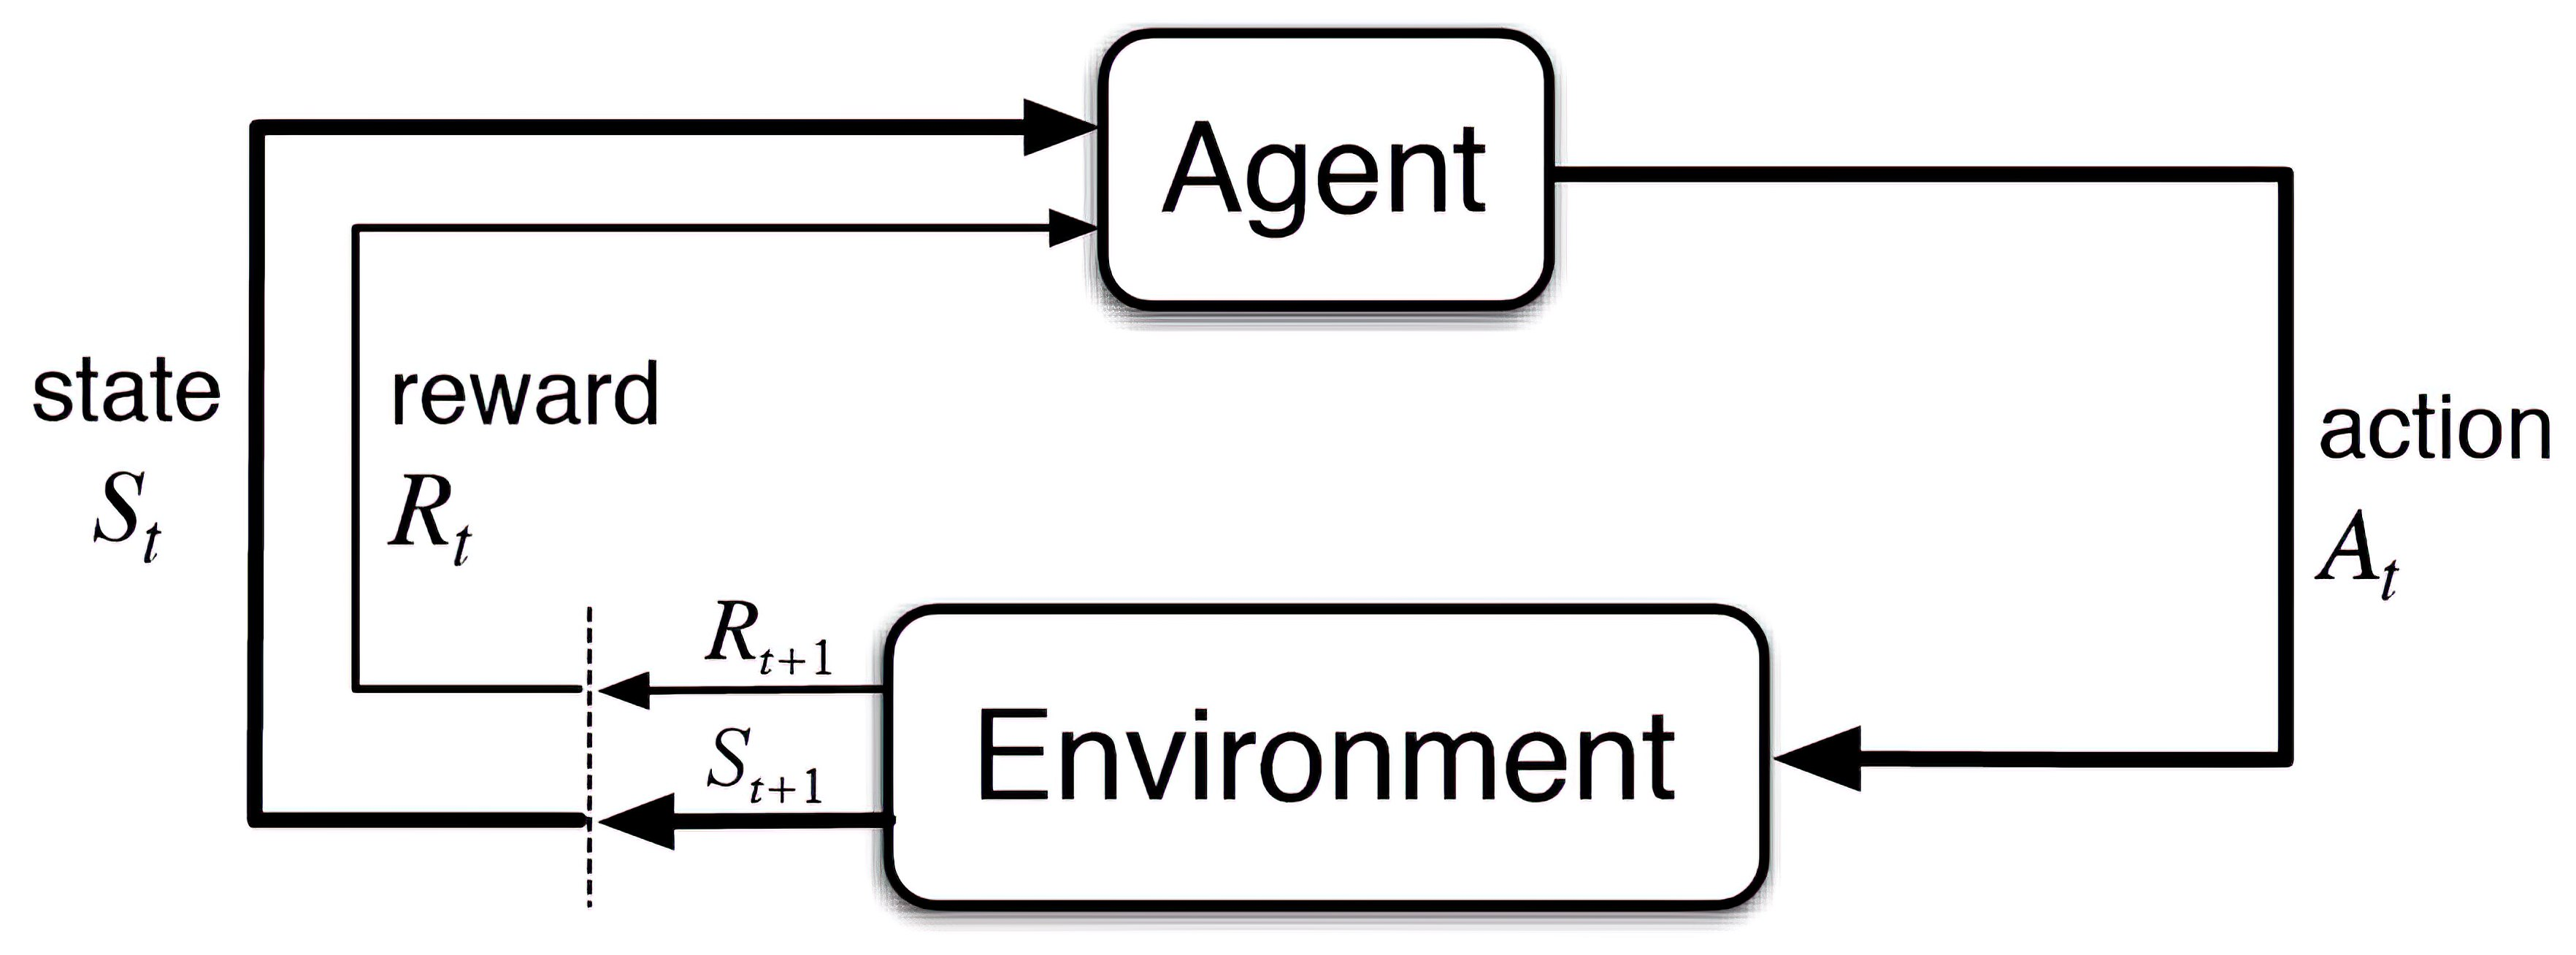
\includegraphics[width = 4in]{Figures/Chapter1/RL_model4x.jpg}
    \caption{Modello del RL}
    \label{fig:rl_model}
\end{figure}

La funzione che in ogni istante di tempo associa ad uno stato una distribuzione di probabilità sull'insieme delle azioni si chiama \textit{policy} e usualmente viene indicata col simbolo $\pi$.

\begin{equation}
	\pi: s \xrightarrow{} \mathcal{D}
\end{equation}

Per misurare la bontà di un'azione $a_t$ eseguita in uno stato $s_t$ viene definita la \textit{action-value function} $Q$ associata alla policy $\pi$

\begin{equation}\label{valueeq1}
	Q^\pi(s_t,a_t) = \mathbb{E}
	\Big[ 
	\sum\limits_{k = 0}^\infty\gamma^k \, r_{t+k}
	\Big]
\end{equation}

mentre per misurare il valore di uno stato $s_t$ si definisce la \textit{state-value function} $V$ associata alla policy $\pi$

\begin{equation}\label{valueev1}
	V^\pi(s_t) = \mathbb{E}
	\Big[ 
	\sum\limits_{k = 0}^\infty\gamma^k \, r_{t+k}
	\Big]
\end{equation}

Dove $\gamma \in [0,1]$ è chiamato \textit{discount factor} e controlla come l'agente valuta le ricompense future nell'ambito dei problemi ad orizzonte infinito\cite{rlSurvey}. Bassi valori favoriscono un comportamento teso a massimizzare le ricompense a breve termine mentre alti valori quelle a lungo termine.\newline

Q è calcolata come la media pesata rispetto a potenze di $\gamma$ delle ricompense future ottenute dall'agente in ottemperanza alla policy $\pi$. L'eq.\ref{valueeq1} è comunemente espressa nella forma di Bellman come segue

\begin{equation}
	Q^\pi(s_t,a_t) = r(s_t,a_t) + \gamma\, Q^\pi(s_{t+1},a_{t+1})
\end{equation}

Dove $r(s_t,a_t)$ è la ricompensa ottenuta nello stato di arrivo $s_{t+1}$ eseguendo l'azione $a_t$ nello stato $s_t$. Per tale motivo verrà indicata anche come $r_{t+1}$.\newline

La tupla $(s_t,a_t,s_{t+1},r_{t+1})$ viene detta \textit{transizione} e rappresenta l'unità fondamentale dell'apprendimento per gli algoritmi di RL nell'ambito dei \textit{Markov Decision Process}.

L'obiettivo dell'agente è imparare una \textit{policy ottima} $\pi^*$, a cui corrisponde una \textit{action-value function} ottima $Q^{\pi^*}$ che calcola il valore di ogni stato $s$ come la somma della ricompensa istantanea e del valore scontato dello stato successivo eseguendo \textit{la migliore azione possibile}

\begin{equation}\label{valueoptimaleq}
	Q^{\pi^*}(s_t,a_t) = r_{t+1} + \gamma \max_{a} Q^{\pi^*}(s_{t+1},a_{t+1}),\, \forall s
\end{equation}

Data la \ref{valueoptimaleq}, la policy ottima si determina come segue

\begin{equation}\label{qtopi}
	\pi^*(s_t) = \argmax_aQ^{\pi^*}(s_t,a_t)
\end{equation}

\clearpage

\subsection{Q-Learning}

Il Q-Learning\cite{qlearningPaper} è uno degli algoritmi model-free\footnote{Classe di algoritmi che non fa utilizzo del modello del processo da ottimizzare ma si basa sul trial-and-error.} più conosciuti del RL e fa parte della famiglia dei Temporal Difference\footnote{Famiglia di algoritmi basati su una ottimizzazione dinamica della stima della action-value function basata sulle osservazioni correnti.}. 

Il cuore dell'algoritmo, che usa la eq.\ref{valueeq1} come action value function, è la funzione di aggiornamento implementata dall'agente:

\begin{equation}
	Q(s_t,a_t) \xleftarrow{} Q(s_t,a_t) + 
	\alpha \,\Big[ r_{t+1} + \gamma\, \max_{a_{t+1}}Q(s_{t+1},a_{t+1}) - Q(s_t,a_t)\Big]
\end{equation}

Dove $\alpha \in [0,1]$ è il \textit{learning rate}, ovvero il tasso con il quale i valori di Q sono aggiornati ad ogni step, e $\gamma$ è quello definito in precedenza.
Sotto l'ipotesi che tutte le azioni sono campionate un numero sufficiente di volte in tutti gli stati e i valori stato-azione sono rappresentati in modo discreto si dimostra\cite{qlearningtecnicalPaper} che il Q-Learning converge con \textit{probabilità 1} alla action-value function ottima $Q^*$.

\clearpage

\section{Deep Reinforcement Learning}

Con l'evoluzione delle \textit{Deep Neural Network} è stato possibile rielaborare i classici algoritmi del RL e di formularne di nuovi. I benefici dell'utilizzo delle DNN come approssimatori di funzioni non lineari sono la possibilità di creare agenti più robusti alle variazioni ambientali e di gestire spazi di stato di dimensioni molto maggiori senza tante complicazioni sulla velocità computazionale.

\subsection{Metodi Value Based}

Questa famiglia di metodi si basa sulla stima della action-value function ottima $Q^*$ come base per poi ricavare una policy ottima $\pi^*$.

\subsubsection{Deep Q-Network}

Il DQN\cite{dqnPaper} è una variante del Q-Learning che implementa una DNN per approssimare la action-value function di eq.\ref{valueeq1}.
\newline

Come si vede dalla fig.\ref{fig:dqnnetwork} la rete riceve in ingresso lo stato attuale e presenta in uscita il \textit{valore} di ogni possibile azione.
Proprio per il fatto che il numero di neuroni in uscita ad una rete neurale non può essere infinito il DQN è utilizzabile solo nel caso di insiemi di azioni numerabili.

\begin{figure}[hb]
    \centering
    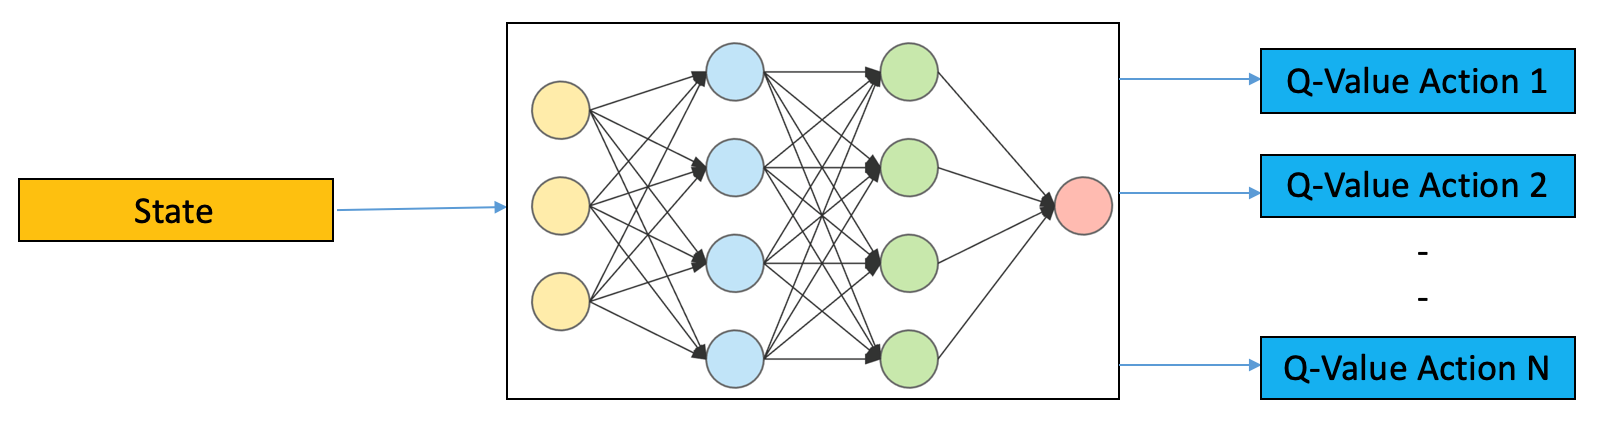
\includegraphics[width = 5.5in]{Figures/Chapter2/dqn.png}
    \caption{Topologia della Deep Q-Network}
    \label{fig:dqnnetwork}
\end{figure}

Per risolvere il problema della divergenza del RL nel caso di utilizzo di approssimatori di funzioni non lineari\cite{rlinstabilityPaper}, gli autori del DQN prevedono l'utilizzo di un \textit{experience replay}, ovvero un buffer dove vengono salvate le transizioni. L'obiettivo di tale aggiunta è che prelevando in maniera casuale le transizioni dal replay buffer si risolve il problema della correlazione tra la sequenza di osservazioni che è una delle cause della divergenza. 
\newline

Ad ogni time step $i$ si prelevano casualmente dall'experience replay un batch $D$ di transizioni e si aggiorna la rete Q seguendo il gradiente della \textit{loss function} di equazione:

\begin{equation}
L(\theta_i) = \mathbb{E}_D 
	\Bigg[ 
	\Big(
	r_{t+1} + \gamma\,\max_{a_{t+1}}Q(s_{t+1},a_{t+1} \,| \,\theta'_i) - Q(s_t,a_t \,| \, \theta_i)
	\Big)^2
	\Bigg]
\end{equation}
	

dove $Q(s_t,a_t \,| \, \theta_i)$ è la rete principale con parametri $\theta_i$ e $Q(s_{t+1},a_{t+1} \,| \,\theta'_i)$ è una seconda rete, detta \textit{target network}, che approssima la action-value function dello stato successivo. I suoi parametri $\theta'_i$ vengono aggiornati con una copia di quelli della main Q-network solo ogni $C$ iterazioni e mantenuti fissi tra gli aggiornamenti.

\clearpage

\subsection{Metodi Policy Based}

In opposizione ai metodi Value Based, questi mirano a stimare direttamente la policy ottima $\pi^*$. Possiamo categorizzarli in \textit{Stochastic Policy Based} o \textit{Deterministic Policy Based}. Il primo tipo di algoritmi produce una distribuzione di probabilità su un insieme numerabile di azioni, mentre il secondo determina direttamente il valore dell'azione da eseguire, e quindi è applicabile a processi con spazi di azioni continui.

\subsubsection{REINFORCE}

REINFORCE\cite{reinforcePaper} è un algoritmo Stochastic Policy Based che utilizza una DNN per implementare una policy $\pi$. Come si evince dalla fig.\ref{fig:reinforce} la rete produce una distribuzione di probabilità sull'insieme di azioni $[a_1,a_2,...,a_k]$ a partire da una osservazione $[s_1,s_2,...,s_N]$.
\newline

\begin{figure}[hb]
    \centering
    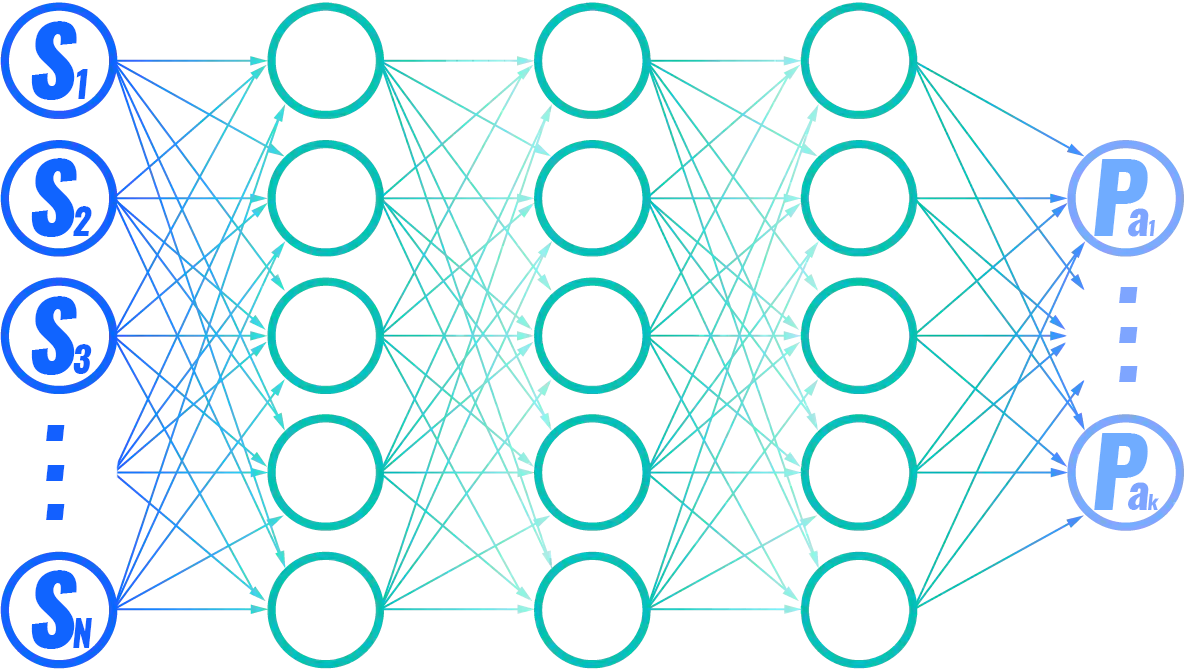
\includegraphics[width = 4in]{Figures/Chapter2/policy_network.png}
    \caption{Policy Network}
    \label{fig:reinforce}
\end{figure}

Il cuore dell'algoritmo è il processo di aggiornamento dei parametri $\theta$ della rete, che viene eseguito a fine di ogni \textit{episodio}\footnote{Un episodio è un insieme di step eseguiti dall'agente fino al raggiungimento di una delle possibili condizioni di terminazione prefissate.}, nella direzione del gradiente della funzione di performance $J(\theta)$ di eq:

\begin{equation}\label{reinforce_perf_eq}
	J(\theta) = \sum_{t=0}^{T-1} \gamma^t \, r_{t+1}
\end{equation}

dove T è il numero di step che compongono l'episodio e il gradiente ha eq:

\begin{equation}\label{reinforce_perf_grad_eq}
	\nabla_{\theta} J(\theta) = \sum_{t=0}^{T-1} \nabla_{\theta} \log \pi_{\theta}(a_t|s_t) \, G(t)
\end{equation}

con $G$ funzione di ricompensa cumulativa scontata di eq: 

\begin{equation}
	G(t) = \sum_{k=0}^{T-t-1} \gamma^k\,r_{t+k+1}
\end{equation}

Ulteriori dettagli sul processo di calcolo della eq.\ref{reinforce_perf_grad_eq} sono reperibili qui\cite{reinforcemathWebsite}.

\clearpage

\subsection{Metodi Actor-Critic}

Questi metodi sono un ibrido che combinano i benefici dei metodi Value Based e di quelli Policy Based. Consistono nell'utilizzo di due DNN, una per la stima della policy $\pi$, nominata \textit{Actor} e una per la stima della \textit{state value function} $V$, nominata \textit{Critic}. Nella fig.\ref{fig:actor-critic} si può osservare il modello.
\newline

\begin{figure}[hb]
    \centering
    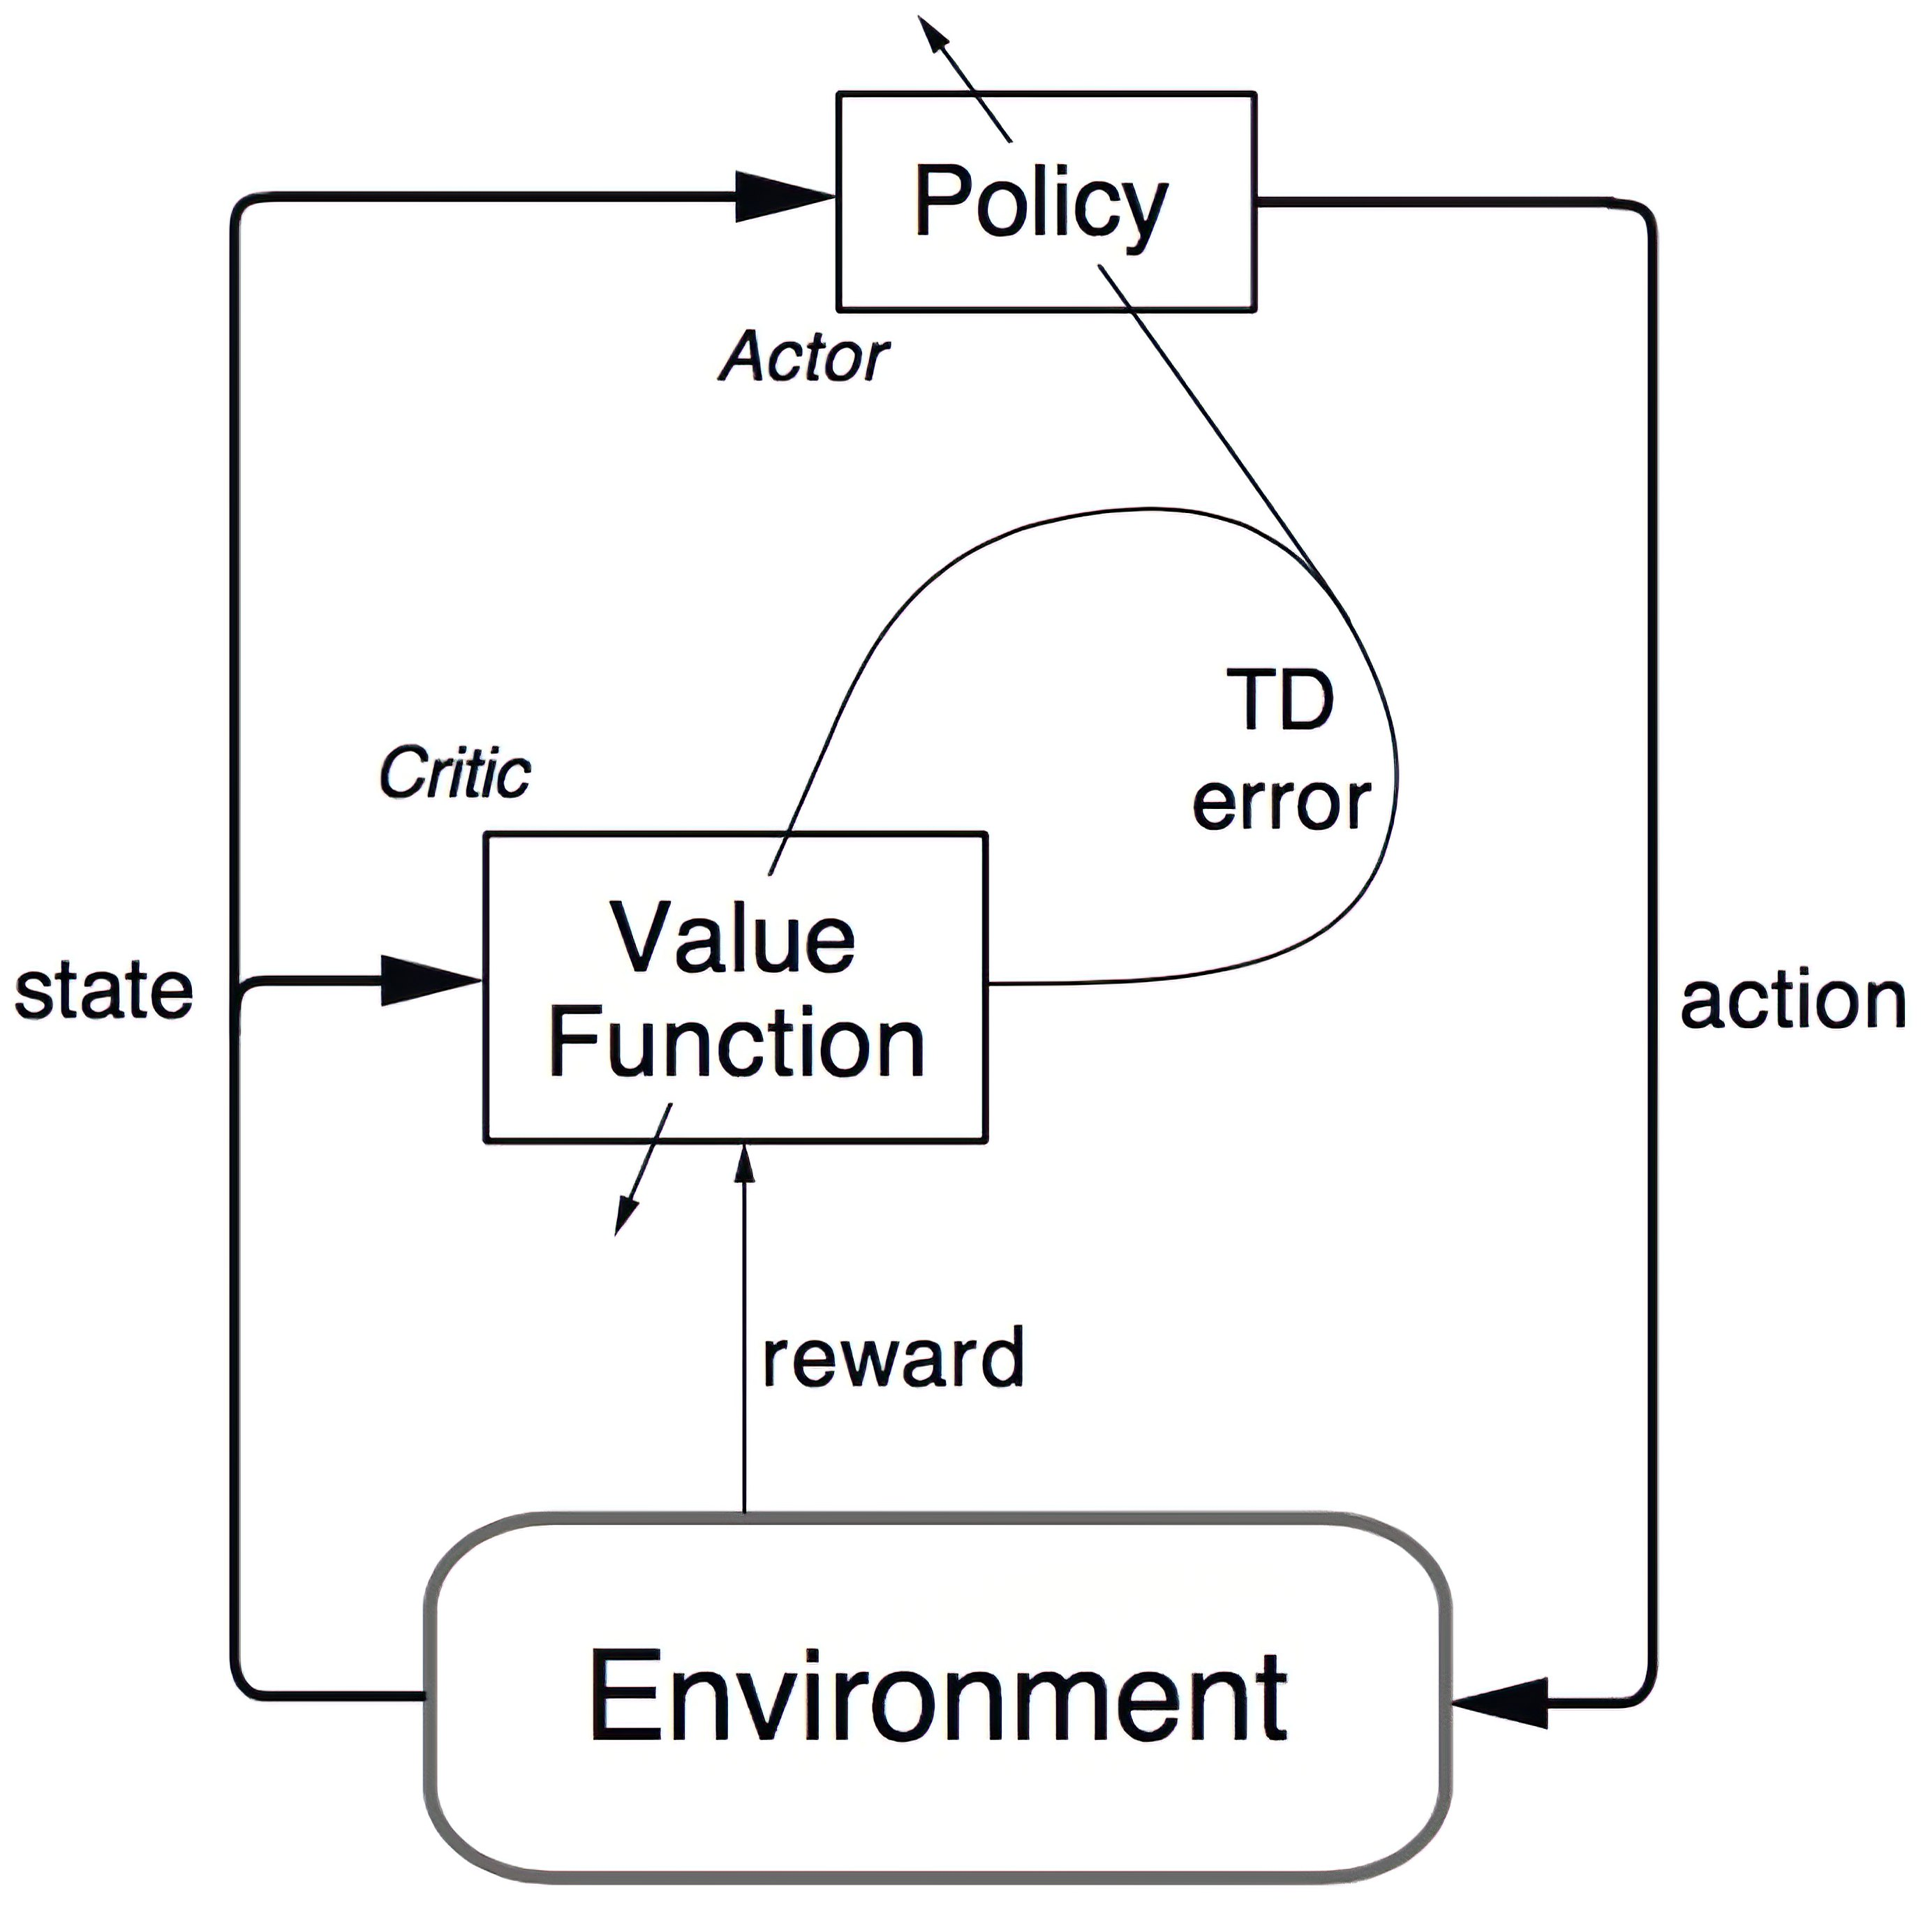
\includegraphics[width = 4in]{Figures/Chapter2/actor-critic_model4x.jpg}
    \caption{Modello dell'Actor-Critic}
    \label{fig:actor-critic}
\end{figure}

Ad ogni step $t$ dell'episodio l'Actor produce un'azione $a_t$ che modifica lo stato dell'ambiente. Il nuovo stato $s_{t+1}$ e la ricompensa associata $r_{t+1}$ vengono poi recepiti dal Critic che ne valuta la bontà attraverso la state-vale function $V_{\theta}(s_{t+1})$ di eq.\ref{valueev1}. Si tenga in considerazione che il Critic mantiene in memoria anche $V_{\theta}(s_t)$ derivante dallo stato precedente.
\newline

L'aggiornamento delle due reti viene fatto ogni step. I parametri $\theta$ della rete Critic vengono aggiornati nella direzione della minimizzazione della seguente funzione di costo:

\begin{equation}
	\delta^2 = \Big[ r_{t+1} + \gamma \, V_{\theta}(s_{t+1}) - V_{\theta}(s_t) \Big]^2
\end{equation}

mentre i parametri $\phi$ dell'Actor vengono aggiornati per minimizzare la funzione di costo:

\begin{equation}
	X = \delta \, \log \pi_{\phi}(a_t|s_t)
\end{equation}

\subsubsection{DDPG}\label{ddpgsection}

Il Deep Deterministic Policy Gradient (DDPG)\cite{ddpgPaper} è un algoritmo model-free e off-policy\footnote{Sono off-policy gli algoritmi che aggiornano i loro parametri basandosi su policy vecchie.}, facente parte della famiglia degli Actor-Critic, che permette ad un agente di imparare una Q-function e una policy \textit{specificatamente} in uno spazio di stato e di azione continuo.
\newline

Questo algoritmo è strettamente connesso al Q-learning ed è motivato allo stesso modo: se si conosce la action-value function ottima $Q^*(s,a)$ allora, in ogni dato stato, la policy ottima può essere trovata risolvendo l'eq.\ref{qtopi}.
\newline

Quando c'è un numero finito di azioni, il calcolo del massimo non pone problemi perché si possono calcolare i Q-value per ogni azione separatamente e successivamente confrontarli. Ma quando lo spazio delle azioni è continuo, non è possibile valutare in modo esauriente il massimo tra i Q-value in quanto si sarebbe costretti a campionare lo spazio d'azione e questo porterebbe inevitabilmente ad errori di valutazione. Inoltre l'utilizzo di un normale algoritmo di calcolo del massimo renderebbe la subroutine estremamente inefficiente all'aumentare del numero delle azioni.
\newline

Tuttavia poiché lo spazio delle azioni è continuo, si presume che la funzione $Q^*(s,a)$ sia differenziabile rispetto all'azione $a$. Questo consente di impostare un apprendimento basato sul gradiente per una policy $\mu(s)$. Quindi, invece di eseguire una costosa subroutine di ottimizzazione ogni volta che si desidera calcolare $\max_{a} Q(s,a)$, è possibile approssimarlo con $Q(s,\mu(s))$.
\newline

Il modello prevede l'utilizzo di due coppie di DNN: 
\begin{itemize}
    \item Una coppia di reti principali: $\mu_{\phi}(s)$, chiamata Actor, che sarà utilizzata per stimare la policy ottima e $Q_{\theta}(s,a)$, chiamata Critic, che stimerà la action-value function ottima.
\item Una seconda coppia di reti: $\mu_{\phi_{targ}}(s)$ e $Q_{\theta_{targ}}(s,a)$, dette \textit{Target Actor} e \textit{Target Critic}, che saranno utilizzate per il calcolo della loss function che permetterà l'aggiornamento dei parametri delle prime due. Queste reti hanno la stessa struttura di quelle principali e vengono aggiornate periodicamente attraverso un \textit{soft update} in base ai loro parametri.
\end{itemize}

Le reti target vengono adoperate in modo che il valore atteso target non sia dipendente dai parametri utilizzati nelle reti principali che calcolano il valore atteso attuale. In questo modo si evitano grosse divergenze tra i due valori migliorando la stabilità durante l’addestramento. Come nel DQN, il DDPG utilizza un experience replay per campionare le esperienze passate e aggiornare i parametri della rete neurale.
\newline

Dato un insieme $D$ di transizioni prelevate dall'experience replay, l'aggiornamento dei parametri della $Q_{\theta}(s,a)$ viene fatta nella direzione di minimizzazione del mean-squared Bellman error (MSBE), che quantifica in che misura $Q_{\theta}$ si avvicina a soddisfare l'equazione di Bellman:

\begin{equation}\label{criticlossddpg}
  L(\theta) = \mathbb{E}_D 
	\Bigg[ 
	\bigg(
	Q_{\theta}(s_t,a_t) - 
	\Big(
	r_{t+1} + \gamma(1-d)Q_{\theta_{targ}}(s_{t+1},\mu_{\phi_{targ}}(s_{t+1}))
	\Big)
	\bigg)^2
	\Bigg]  
\end{equation}

con $d$ un flag booleano posto ad 1 quando $s_{t+1}$ è uno stato terminale, in modo che la Q-function non attribuisca ulteriore valore all'azione se non quella conferita dalla ricompensa immediata $r_{t+1}$.
\newline

L'aggiornamento dei parametri dell'Actor è più intuitivo in quanto viene fatto seguendo la massimizzazione della funzione $Q_{\theta}(s_t,\mu_{\phi}(s))$ rispetto i sui parametri $\phi$, e quindi nella direzione del gradiente:

\begin{equation}\label{gradactorddpg}
   \nabla_{\phi} \, Q_{\theta}(s_t,\mu_{\phi}(s)) =
   \frac{\partial}{\partial \mu_{\phi}} \, Q_{\theta}(s_t,\mu_{\phi}(s)) \,
   \frac{\partial}{\partial\phi} \, \mu_{\phi}(s)
\end{equation}


I parametri delle reti target vengono aggiornati seguendo un \textit{soft update}:

\begin{equation}\label{ddpgsoftupdate_eq}
   \begin{aligned}
       &\theta_{targ} \xleftarrow{} \tau \theta + (1-\tau) \theta_{targ} \\
       &\phi_{targ} \xleftarrow{} \tau \phi + (1-\tau) \phi_{targ}
   \end{aligned}
\end{equation}

dove $\tau$ è detto \textit{smooth factor} e generalmente è molto piccolo per garantire un aggiornamento lento delle reti target.

\clearpage

Di seguito viene mostrato lo pseudocodice dell'algoritmo DDPG\cite{ddpgPaper}:

\begin{figure}[hb]
    \centering
    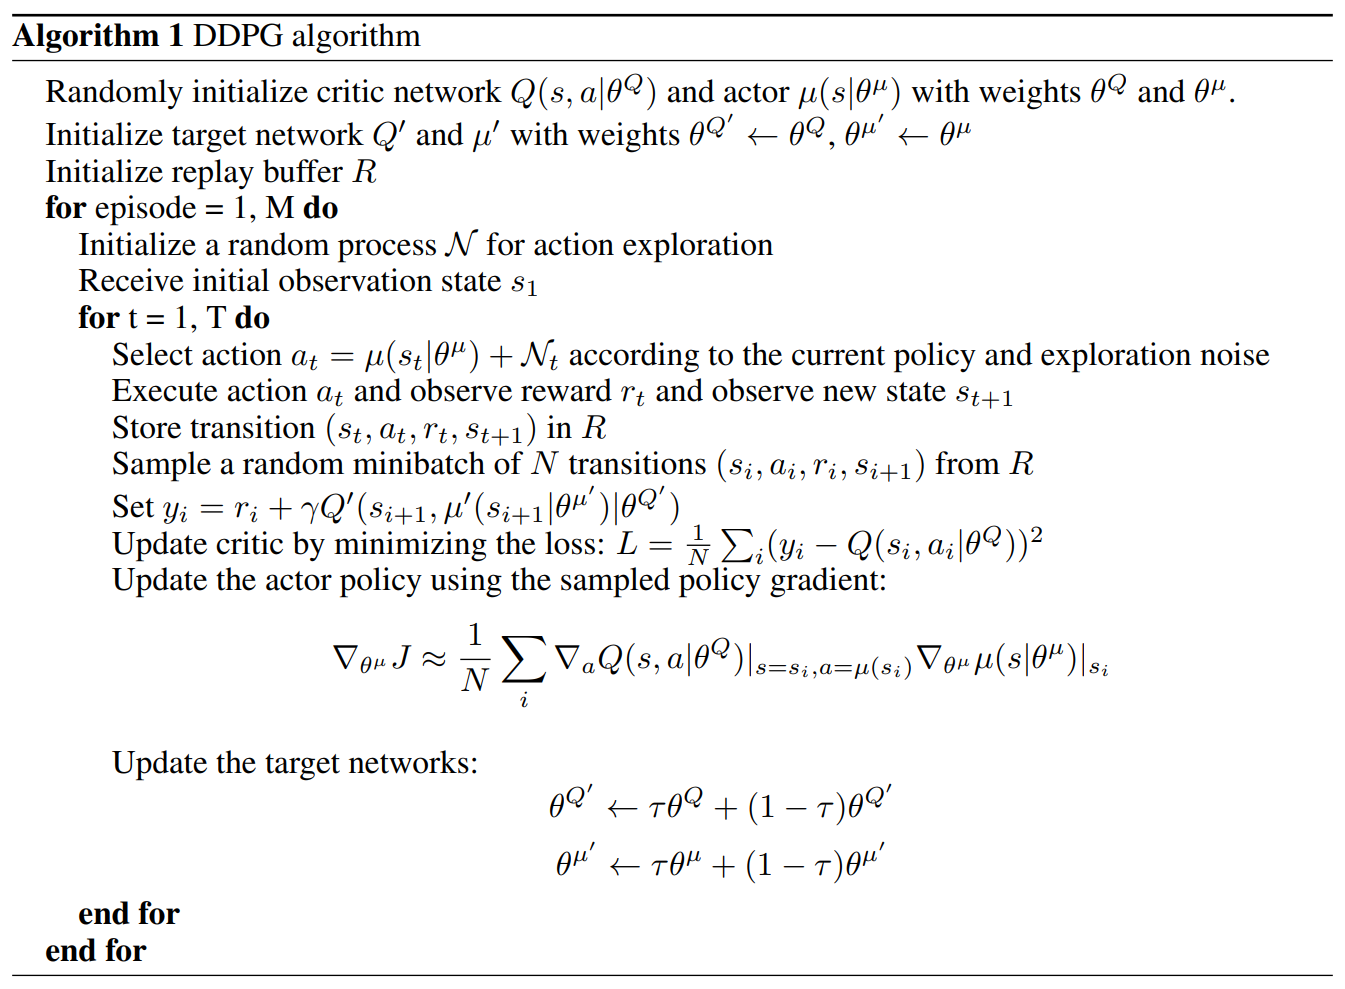
\includegraphics[width = 6in]{Figures/Chapter2/ddpg_algo.png}
    \caption{Algoritmo DDPG}
    \label{fig:ddpgalgo}
\end{figure}

\clearpage
\chapter{Problem Statement}

Per risolvere il problema dell'Autonomous Driving (AU) di un veicolo terrestre, esso, normalmente, viene scomposto in diversi sotto problemi, ognuno dei quali viene risolto da uno specifico processo. Ad esempio, l'\textit{Obstacle Avoidance} è il processo che risolve la gestione degli ostacoli presenti sul percorso durante la guida, oppure l'\textit{Overtaking} è quello che si occupa di gestire il sorpasso di altri veicoli.
\newline

Tutti questi processi, però, fondano il loro corretto funzionamento sul fatto che, in principio, l'auto si trovi correttamente in carreggiata durante tutto il processo di guida. Il processo che risolve questo fondamentale problema viene detto \textit{Lane Keeping}.
\newline

I tradizionali sistemi di AU sono basati su regole precostruite e devono creare informazioni sulla struttura dalle scene prima di prendere una decisione. Le informazioni sulla struttura sono molto complicate, il che porta alla costruzione di regole complesse e quindi ad una difficile costruzione di un modello decisionale completo ed efficace.
Con gli ultimi sviluppi dell'Intelligenza Artificiale nell'AU è stato possibile affidare la comprensione di scene complesse e il processo decisionale alle reti neurali senza bisogno di regole definite dall'uomo. In queste circostanze è comune parlare di sistema decisionale end-to-end\footnote{Un sistema che produce una decisione direttamente a partire dalla comprensione dell'ambiente, senza passaggi intermedi.}.
\newline

L'obiettivo di questa tesi è quello di affrontare il problema del lane keeping nell'ambiente avanzato di simulazione di guida TORCS\cite{torcsWebsite}, attraverso un sistema decisionale end-to-end basato sul DDPG. Il lavoro si ispira a quello dei ricercatori della \textit{Beijing University of Technology}\cite{mainTORCSPaper}.


\section{Introduzione a TORCS}

TORCS\cite{torcsWebsite} è un simulatore 3D di gare automobilistiche open source. Esso è progettato per permettere a delle IA pre-programmate di gareggiare le une contro le altre e permette ad un giocatore di utilizzare una tastiera, un mouse, o un volante per controllare un veicolo.

\begin{figure}[hb]
    \centering
    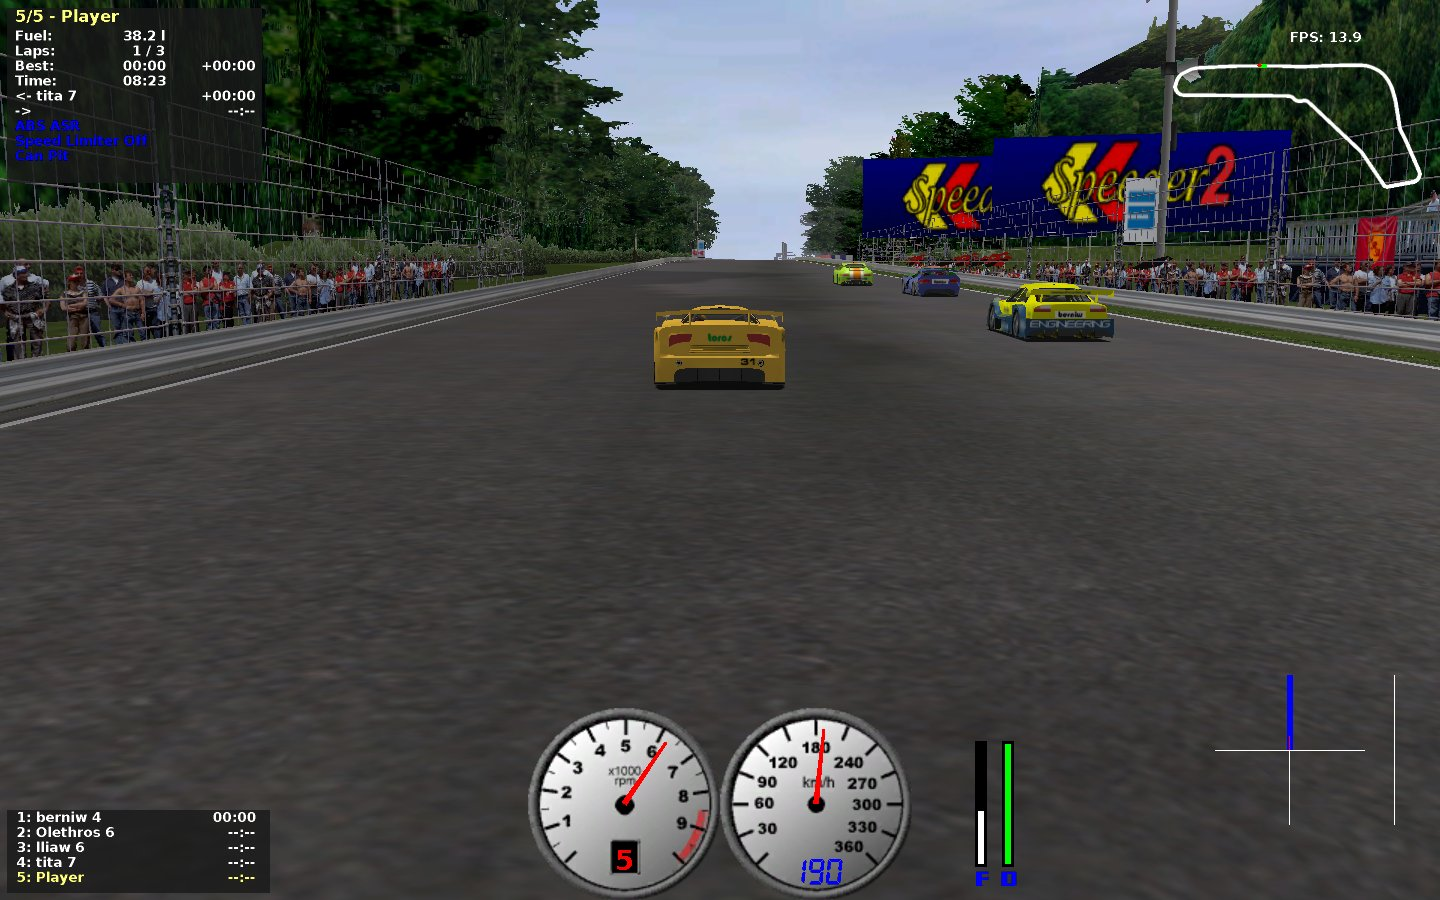
\includegraphics[width = 5in]{Figures/Chapter3/torcs_game.jpg}
    \caption{Immagine di una gara in TORCS}
    \label{fig:torcsgame}
\end{figure}

TORCS si presenta come un'applicazione autonoma in cui i bot vengono compilati come moduli separati che vengono caricati nella memoria principale quando si svolge una gara. Questo presenta diversi svantaggi sul profilo della realizzazione in quanto impone la modalità di interfacciamento col gioco e il linguaggio di programmazione da utilizzare.
\newline

Nell'ambito di questa tesi si è utilizzata la versione di TORCS con patch SCR.
\newline

Simulated Car Racing (SCR)\cite{scrloiaconoPaper} estende l'architettura TORCS originale sotto tre aspetti. Innanzitutto struttura TORCS come un'applicazione Client-Server: i bot vengono eseguiti come processi esterni connessi al server di gara tramite connessioni UDP. 

In secondo luogo, aggiunge il real-time: ad ogni tic di gioco (corrispondente all'incirca a 20 ms di tempo simulato), il server invia gli input sensoriali correnti a ciascun bot
e poi attende 10ms (di tempo reale) per ricevere un'azione dal bot. Se non arriva nessuna azione la simulazione continua e viene utilizzata l'ultima azione eseguita. 

Infine SCR costruisce un livello d'astrazione che garantisce una separazione fisica tra il codice dell'AI di guida  e il server di gara, \textit{un modello di sensori e attuatori}, che lascia completa libertà di scelta in merito al linguaggio di programmazione utilizzato per i bot.
\newline

Nella figura seguente viene mostrata l'architettura di SCR.

\begin{figure}[hb]
    \centering
    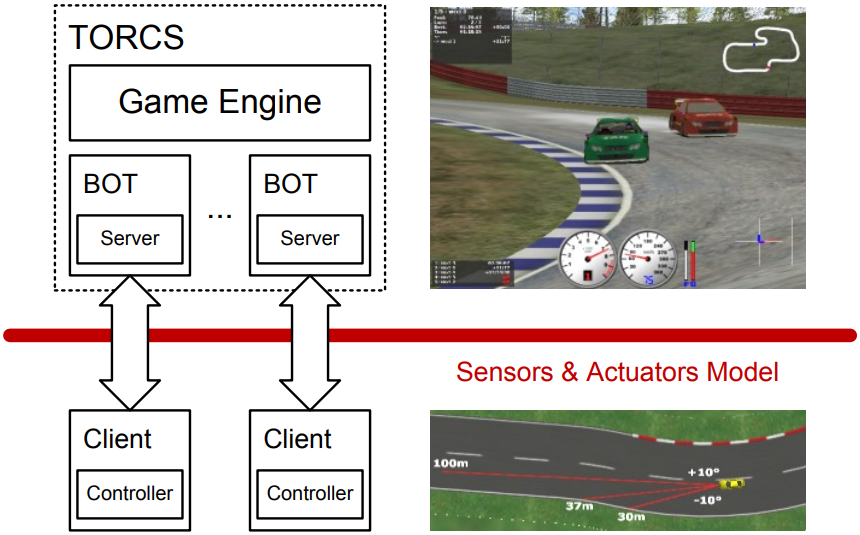
\includegraphics[width = 4in]{Figures/Chapter3/scr_model.png}
    \caption{Architettura di SCR}
    \label{fig:scrmodel}
\end{figure}

La lista completa dei sensori e degli attuatori forniti da SCR non è riportata per brevità ma è consultabile in\cite{scrloiaconoPaper}.

\clearpage

\section{Segnali di interazione con l'ambiente}

In questo lavoro si presenta un agente capace di terminare il percorso di gara, rimanendo sempre in carreggiata, utilizzando un sottoinsieme dei sensori forniti da TORCS. Nella tab.\ref{tab:statetable} sono definiti i sensori utilizzati per costruire lo stato $s$ mentre nella tab.\ref{tab:actiontable} gli attuatori, ovvero l'azione $a$ che l'agente può eseguire sull'ambiente.

\begin{table}[hb]
\centering
\begin{tabular}{|ccl|}
\hline
\multicolumn{1}{|l|}{{\color[HTML]{000000} \textbf{Nome}}} &
  \multicolumn{1}{c|}{{\color[HTML]{000000} \textbf{Range (unità)}}} &
  \multicolumn{1}{c|}{{\color[HTML]{000000} \textbf{Descrizione}}} \\ \hline
\multicolumn{1}{|c|}{{\color[HTML]{000000} angle}} &
  \multicolumn{1}{c|}{{\color[HTML]{000000} $[-\pi,+\pi] (rad) \in \mathbb{R}$}} &
  {\color[HTML]{000000} \begin{tabular}[c]{@{}l@{}}Angolo tra la direzione dell'auto \\ e l'asse della carreggiata\end{tabular}} \\ \hline
\multicolumn{1}{|c|}{{\color[HTML]{000000} speedX}} &
  \multicolumn{1}{c|}{{\color[HTML]{000000} $[0,300] (km/h) \in \mathbb{R}$}} &
  {\color[HTML]{000000} \begin{tabular}[c]{@{}l@{}}Velocità dell'auto lungo il suo asse longitudinale\end{tabular}} \\ \hline
\multicolumn{1}{|c|}{speedY} &
  \multicolumn{1}{c|}{$[0,300] (km/h) \in \mathbb{R}$} &
  \begin{tabular}[c]{@{}l@{}}Velocità dell'auto lungo il suo asse trasversale\end{tabular} \\ \hline
\multicolumn{1}{|c|}{speedZ} &
  \multicolumn{1}{c|}{$[0,300] (km/h) \in \mathbb{R}$} &
  \begin{tabular}[c]{@{}l@{}}Velocità dell'auto lungo il suo asse Z\end{tabular} \\ \hline
\multicolumn{1}{|c|}{track} &
  \multicolumn{1}{c|}{$[0,200] (m) \in \mathbb{R}^{19}$} &
  \begin{tabular}[c]{@{}l@{}}Vettore di 19 rangefinder disposti a diverse\\ angolazioni davanti l'auto: ogni sensore\\ misura la distanza tra l'auto e il bordo \\ della carreggiata in un range di 200 metri\end{tabular} \\ \hline
\multicolumn{1}{|c|}{trackPos} &
  \multicolumn{1}{c|}{$[-1,+1] \in \mathbb{R}$} &
  \begin{tabular}[c]{@{}l@{}}Distanza normalizzata tra l'auto \\ e l'asse della carreggiata\end{tabular} \\ \hline
\end{tabular}
\caption{Sensori utilizzati nella costruzione del vettore di stato}
\label{tab:statetable}
\end{table}


\begin{table}[hb]
\centering
\begin{tabular}{|ccl|}
\hline
\multicolumn{1}{|l|}{{\color[HTML]{000000} \textbf{Nome}}} &
  \multicolumn{1}{c|}{{\color[HTML]{000000} \textbf{Range (unità)}}} &
  \multicolumn{1}{c|}{{\color[HTML]{000000} \textbf{Descrizione}}} \\ \hline
\multicolumn{1}{|c|}{{\color[HTML]{000000} accel}} &
  \multicolumn{1}{c|}{{\color[HTML]{000000} $[0,1] \in \mathbb{R}$}} &
  {\color[HTML]{000000} \begin{tabular}[c]{@{}l@{}}Pedale del gas virtuale  (0 significa accelerazione\\ nulla e 1 accelerazione massima)\end{tabular}} \\ \hline
\multicolumn{1}{|c|}{{\color[HTML]{000000} brake}} &
  \multicolumn{1}{c|}{{\color[HTML]{000000} $[0,1] \in \mathbb{R}$}} &
  {\color[HTML]{000000} \begin{tabular}[c]{@{}l@{}}Pedale del freno virtuale (0 significa frenata\\ nulla e 1 frenata massima)\end{tabular}} \\ \hline
\multicolumn{1}{|c|}{steer} &
  \multicolumn{1}{c|}{$[-1,+1] \in \mathbb{R}$} &
  \begin{tabular}[c]{@{}l@{}}Sterzo virtuale (-1 significa sterzata massima\\ a destra e +1 sterzata massima a sinistra)\\ Sterzata massima di $0,366519 \, rad$\end{tabular} \\ \hline
\end{tabular}
\caption{Azioni eseguibili dall'agente}
\label{tab:actiontable}
\end{table}

Nella modellazione si è scelto di direzionare i 19 rangefinder nelle seguenti angolazioni: (-45, -19, -12, -7, -4, -2.5, -1.7, -1, -0.5, 0, 0.5 , 1, 1.7, 2.5, 4, 7, 12, 19, 45) gradi. In definitiva lo spazio di stato dell'agente è $s \in \mathbb{R}^{24}$ e quello di azione è $a \in \mathbb{R}^{3}$.

\clearpage
\chapter{Design del Controllo}

Il modello del controllo scelto si basa sul DDPG (presentato nella sez. \ref{ddpgsection}). In questo capitolo ci si soffermerà sulla particolarizzazione dell'algoritmo nel caso di applicazione specifico.
\newline

L'obiettivo dell'agente, in questo caso, è quello di far rimanere sempre in carreggiata l'auto, mentre cerca di farle completare il percorso più velocemente possibile, in uno scenario ad agente singolo. 

Il modello dell'intero sistema di fig.\ref{fig:system_model} mostra le interazioni tra agente ed environment TORCS.
\newline

Il flusso del sistema può essere diviso in due parti fondamentali che avvengono simultaneamente ad ogni istante di tempo $t$:
\begin{enumerate}
    \item \textit{Esplorazione:} A partire da una osservazione $s_t$ la rete Actor $\mu_{\phi}$ produce un'azione $a_t=\mu_{\phi}(s_t)$, con $a_t=(a_{accel},a_{brake},a_{steer}) \in \mathbb{R}^3$. A questa azione viene aggiunto un \textit{rumore esplorativo} e il risultato viene poi inviato a TORCS che restituisce lo stato successivo $s_{t+1}$. Dallo stato successivo si calcola la ricompensa immediata $r_{t+1}$. La transizione del sistema $(s_t,a_t,s_{t+1},r_{t+1})$ viene infine memorizzata nell'experience replay per l'allenamento dell'agente.
    \item \textit{Allenamento:} Viene prelevato un batch di transizioni dal buffer. I parametri della rete Critic $Q_{\theta}$ vengono aggiornati seguendo la loss di eq.\ref{criticlossddpg}. L'Actor, successivamente, viene aggiornato secondo il gradiente di eq.\ref{gradactorddpg}. Infine i parametri delle reti target vengono aggiornati tramite soft update seguendo la eq.\ref{ddpgsoftupdate_eq}.
\end{enumerate}

\begin{figure}[hb]
    \center
    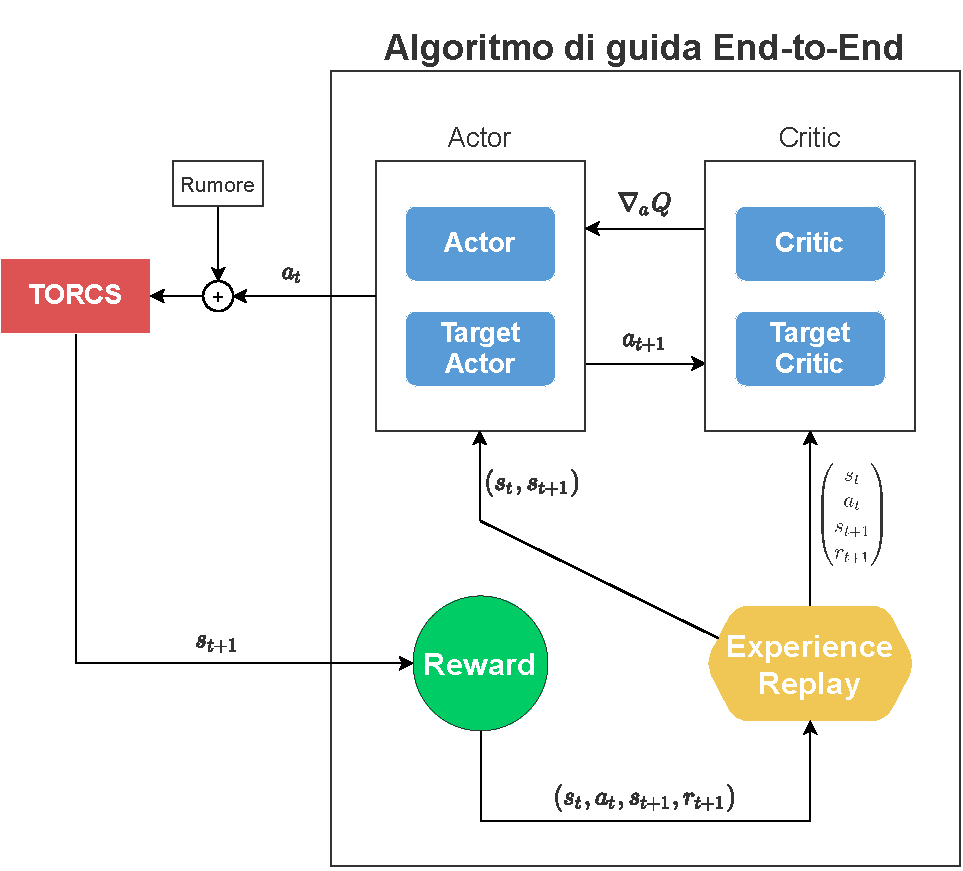
\includegraphics[width = 6in]{Figures/Chapter4/model_ddpg.drawio.pdf}
    \caption{Modello del sistema TORCS-Agente}
    \label{fig:system_model}
\end{figure}

\clearpage

\section{Architettura delle reti}

In questa sezione vengono definite le architetture delle reti utilizzate.
\newline

La rete Actor di fig.\ref{fig:actor_network} è una rete \textit{fully connected} con un input di 24 neuroni, che rappresentano lo stato, e un output di 3 neuroni, ovvero le azioni. I due neuroni che producono l'uscita di \textit{accel} e \textit{brake} sono attivati con \textit{sigmoide} per garantire un output compreso in $[0,1]$, mentre il neurone che produce l'azione di \textit{steer} viene attivato dalla \textit{tangente iperbolica} in modo da avere un range di uscita compreso in $[-1,+1]$. Frapposti tra i livelli di ingresso e uscita ci sono due livelli nascosti da 300 e 400 neuroni con attivazione relu.



\begin{figure}[hb]
    \center
    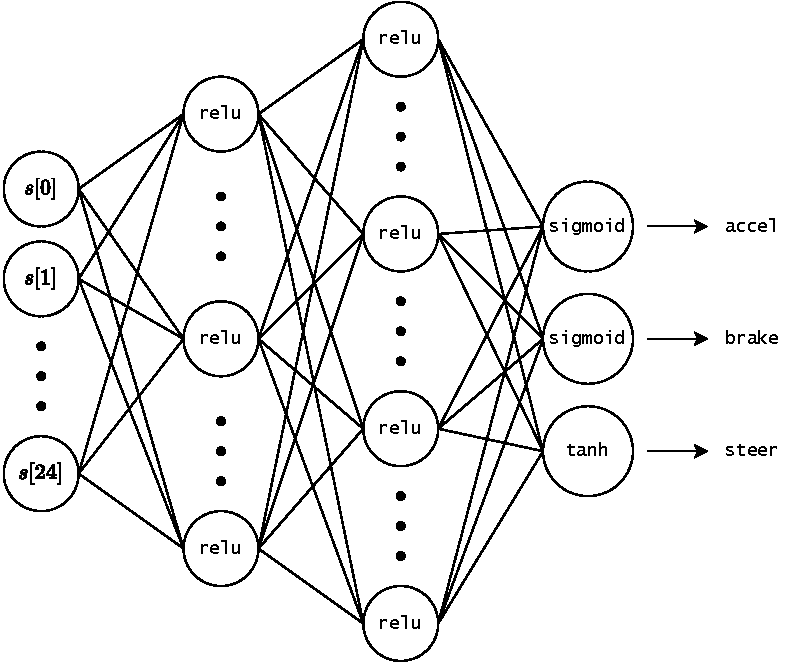
\includegraphics[width = 3.5in]{Figures/Chapter4/ddpg_actor_network.drawio.pdf}
    \caption{Rete Actor}
    \label{fig:actor_network}
\end{figure}

\clearpage

La struttura della rete Critic è mostrata in fig.\ref{fig:critic_network}. L'input è diviso in due parti, una è l'informazione sullo stato dell'ambiente fornita da TORCS e l'altra è il valore dell'azione emesso dalla rete Actor. Le informazioni sullo stato ambientale vengono elaborate dal primo livello nascosto, combinate con il valore dell'azione e inserite nel secondo livello nascosto. I due livelli includono rispettivamente 300 e 400 neuroni e sono attivati da funzione relu. Infine il risultato viene elaborato dal neurone di output per ottenere il Q-value.

\begin{figure}[hb]
    \center
    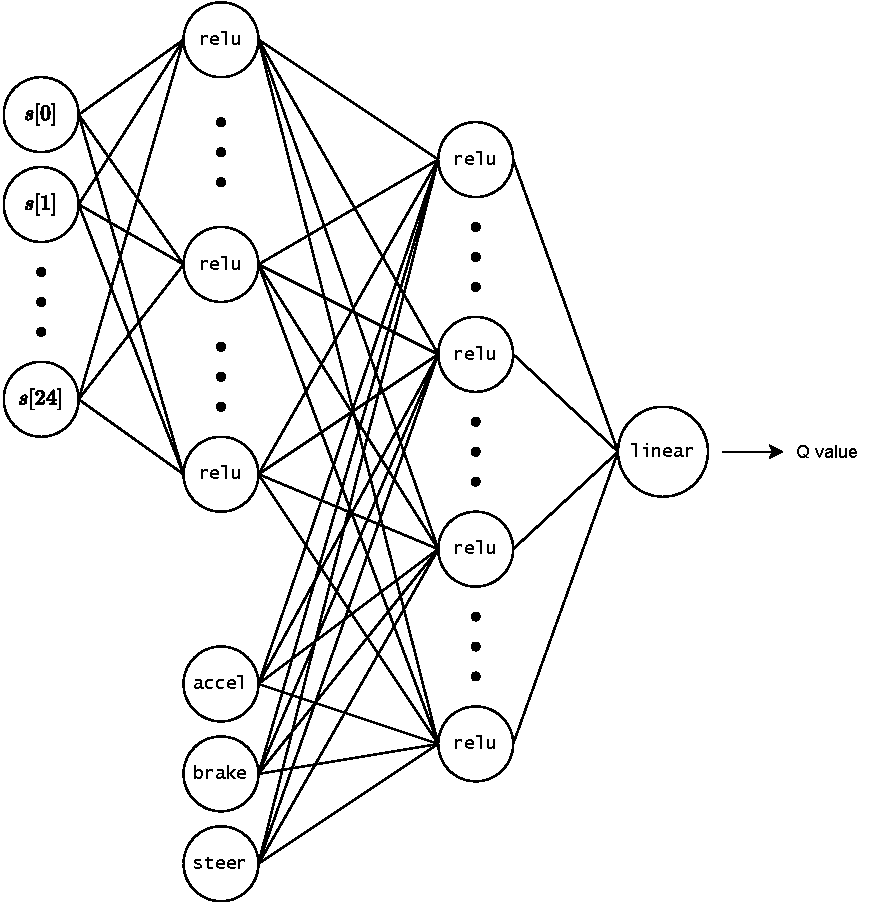
\includegraphics[width = 3.5in]{Figures/Chapter4/ddpg_critic_network.drawio.pdf}
    \caption{Rete Critic}
    \label{fig:critic_network}
\end{figure}

\clearpage

\section{Reward Shaping}

Come viene spiegato nel capitolo introduttivo del RL, la ricompensa è ciò che più di ogni altra cosa caratterizza l'apprendimento dell'agente. Essa infatti definisce \textit{cosa l'agente imparerà e come}.
\newline

L'obiettivo in questo caso è mantenere il veicolo al centro della corsia e terminare il percorso più velocemente possibile. La ricompensa sarà quindi funzione della velocità e dell'offset tra l'agente e il centro della corsia. Nella eq.\ref{rewardfunction} si definisce la funzione di ricompensa, dove le variabili sono definite nella tab. \ref{tab:statetable}.

\begin{equation}\label{rewardfunction}
r =
\begin{cases}
   S_x \, cos(\alpha) - |S_x \, sin(\alpha)| - |S_x \, \gamma| & \text{se } |\gamma|<1\\
   -200                                                        & \text{se } |\gamma|>1
\end{cases}
\end{equation}

con $S_x=speedX$, $\alpha=angle$ e $\gamma=trackPos$.
\newline

Oltre alla reward sopra definita sono state testate anche delle sue varianti. Una prima variante senza il controllo puntuale della trackPos, definita nella eq.\ref{rewardfunction_notrackpos}, e una sostituendo il controllo della trackPos con un controllo dell'angolo dell'auto rispetto alla carreggiata, definita nella eq.\ref{rewardfunction_angle}.

\begin{equation}\label{rewardfunction_notrackpos}
r =
\begin{cases}
   S_x \, cos(\alpha) - |S_x \, sin(\alpha)| & \text{se } |\gamma|<1\\
   -200                                      & \text{se } |\gamma|>1
\end{cases}
\end{equation}

\begin{equation}\label{rewardfunction_angle}
r =
\begin{cases}
   S_x \, cos(\alpha) - |S_x \, sin(\alpha)| - S_x\big|\frac{\alpha}{\pi}\big| & \text{se } |\gamma|<1\\
   -200                                                                        & \text{se } |\gamma|>1
\end{cases}
\end{equation}

\clearpage

\section{Rumore Esplorativo}

Negli algoritmi di Deep RL devono essere impostate strategie di esplorazione appropriate per evitare che l'algoritmo cada in un ottimo locale. Questo problema è comunemente noto come l'\textit{Explore-Exploit Dilemma}. 
\newline

\textit{L'Explore} consiste nella scelta di un'azione casuale. Ciò consente all'agente di migliorare le proprie conoscenze attuali sugli action-value, con un possibile vantaggio a lungo termine. 
Il miglioramento dell'accuratezza degli action-value stimati gli consentirà di prendere decisioni più informate in futuro. \textit{L'Exploit}, d'altra parte, sceglie l'azione avidamente per ottenere la massima ricompensa sfruttando le attuali stime delle action-value conosciute. 
Quando un agente esplora tende a costruire stime mano a mano più accurate degli action-value e quando sfrutta mira ad ottenere più ricompense. Non può, tuttavia, scegliere di fare entrambe le cose contemporaneamente. Per tale ragione è necessario utilizzare tecniche per la gestione delle fasi di esplorazione e sfruttamento.
\newline

In base all'algoritmo utilizzato esistono tecniche esplorative differenti. Nel caso del DQN, una nota strategia esplorativa è l'$\epsilon$-greedy, che consiste nell'eseguire un'azione casuale con probabilità $\epsilon$ e un'azione che massimizzi la $Q$ con probabilità $(1-\epsilon)$.
\newline

Strategie di esplorazione comuni come $\epsilon$-greedy non sono adatte a scenari di guida autonoma come quello esaminato in questa tesi perché si presenterebbero molti casi di azioni invalide, come ad esempio azioni in cui la frenata è maggiore dell'accelerazione.
\newline

Per tale ragione l'autore del DDPG propone l'utilizzo di un rumore additivo sull'azione generato dal processo stocastico di Ornstein-Uhlenbeck\cite{ddpgPaper}. Nell'ambito di questo lavoro sono stati testati tre tipi di rumori esplorativi: una variante dell'\textit{Ornstein-Uhlenbeck}, un \textit{Gaussian Noise} e un \textit{Time Variant Noise}. Questi rumori vengono presentati nelle seguenti sottosezioni.

\clearpage

\subsection{Ornstein-Uhlenbeck Mod}

Questo rumore è una variazione dell'\textit{Ornstein-Uhlenbeck} in quanto nel 10\% dei casi viene prodotto un rumore gaussiano $N(\mu,\sigma)$ mentre nel 90\% dei casi viene prodotto un rumore in base al classico processo stocastico di Ornstein-Uhlenbeck.
\newline

Questo serve a fare in modo che l'agente sia sollecitato con due stimoli molto diversi fra loro in misure diverse. Nove volte su dieci si stimola l'agente ad andare molto veloce attraverso un rumore additivo con media alta sull'accelerazione e nulla sulla frenata e, una volta su dieci, invece, lo si stimola a frenare attraverso un rumore con una media nettamente inferiore sull'accelerazione e alta sulla frenata.

\subsection{Gaussian Noise}

Questo rumore è una variazione dell'\textit{$\epsilon$-greedy Gaussian Noise} in quanto nel 90\% dei casi viene prodotto un rumore gaussiano $N(\mu_1,\sigma_1)$ mentre nel 10\% dei casi uno $N(\mu_2,\sigma_2)$. 
\newline

Anche in questo caso si utilizza questo stratagemma, con un opportuno tuning dei parametri di medie e std, per sollecitare l'agente con stimoli molto diversi fra loro per garantire che esso impari un più ampio spettro di comportamenti.
\newline

La probabilità $\epsilon$ viene fatta decadere linearmente rispetto al numero delle iterazioni di training.

\clearpage

\subsection{Time Variant Noise}

Il TVNoise è un rumore gaussiano con media e std variabile nel tempo.
La classe restituisce un rumore gaussiano $N(\mu_1,\sigma_1)$ per i primi \textbf{\texttt{time\_step1}} passi.
\newline

Successivamente tende linearmente ad un rumore con distribuzione gaussiana $N(\mu_2,\sigma_2)$ in un numero di passi pari a \\\textbf{\texttt{(self.time\_step2 - self.time\_step1)}}.
\newline

Infine, sempre linearmente, tende a $N(\mu_3,\sigma_3)$ in \textbf{\texttt{(self.time\_step3 - self.time\_step2)}} passi. Nel progetto di tesi questo terzo passaggio viene sfruttato per far decadere a zero linearmente il rumore gaussiano aggiunto.
\newline

Nella fig.\ref{fig:tv_noise_media} viene mostrato un esempio di possibile andamento della media del rumore gaussiano. Lo stesso ragionamento si applica alla std.

\begin{figure}[hb]
    \center
    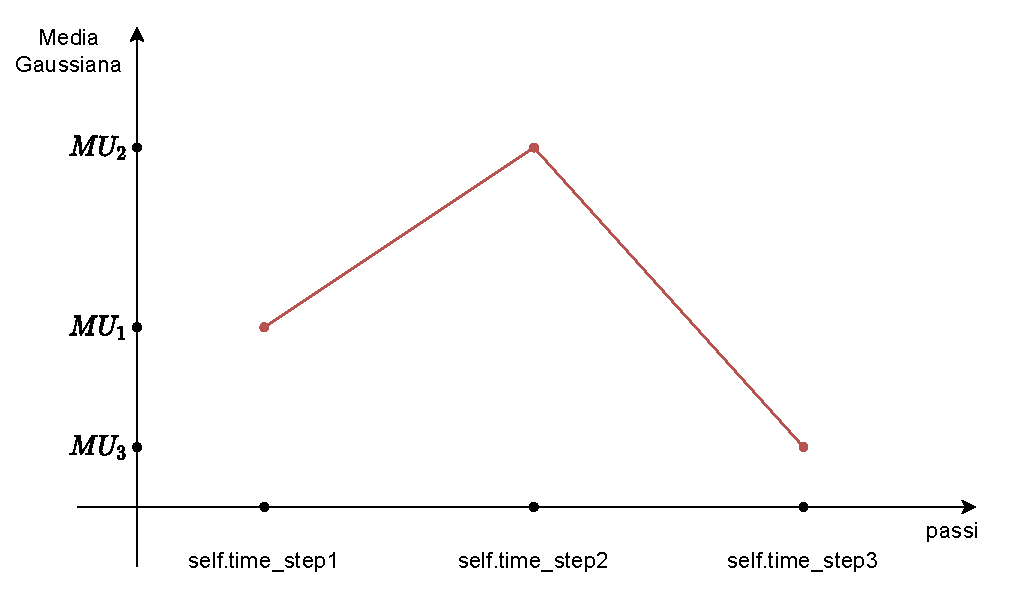
\includegraphics[width = 5in]{Figures/Appendix/tvnoise_media.drawio.pdf}
    \caption{Andamento della media Gaussiana}
    \label{fig:tv_noise_media}
\end{figure}
\chapter{Simulazioni e Risultati}
\section{Set-up Numerico}
In questo capitolo si discutono le simulazioni effettuate e si analizzano i risultati con l'obiettivo di trovare il miglior modello, sia rispetto agli episodi di allenamento, sia rispetto agli altri modelli che presentano parametri diversi. Per affrontare in maniera consistente questo processo, si definiscono nella tab.\ref{tab:model_params} i parametri che caratterizzano nell'interezza un modello DDPG e nella tab.\ref{tab:model_metrics} le metriche utilizzate nel giudizio di questi ultimi.
\newline

Nella fig.\ref{fig:tracks} si vede a sinistra il tracciato utilizzato per il training dei modelli e a destra quello utilizzato per la validazione.

\begin{figure}[hb]
    \centering
    
\includegraphics[width = 3.5in]{Figures/Chapter5/training_test_track.png}
    \caption{Tracciati di training e validazione}
    \label{fig:tracks}
\end{figure}

\clearpage


\begin{table}[hb]
\centering
\begin{tabular}{|cl|}
\hline
\multicolumn{1}{|c|}{\textbf{Nome}}  & \multicolumn{1}{c|}{\textbf{Descrizione}}                                                                                    \\ \hline
\multicolumn{1}{|c|}{MEM\_SIZE}      & Dimensione dell'experience replay                                                                                            \\ \hline
\multicolumn{1}{|c|}{BATCH\_SIZE}    & \begin{tabular}[c]{@{}l@{}}Dimensione del batch di transizioni prelevate\\ contemporaneamente dall'experience replay\end{tabular} \\ \hline
\multicolumn{1}{|c|}{DC\_FACT}       & Discount Factor $\gamma$ del Q Learning                                                                         \\ \hline
\multicolumn{1}{|c|}{SM\_FACT}       & Fattore di smooth $\tau$ utilizzato nel soft update                                                             \\ \hline
\multicolumn{1}{|c|}{CLR}            & Learning rate del Critic e del Target Critic                                                                                 \\ \hline
\multicolumn{1}{|c|}{ALR}            & Learning rate dell'Actor e del Target Actor                                                                                  \\ \hline
\multicolumn{1}{|c|}{C\_1} & \begin{tabular}[c]{@{}l@{}}Numero di neuroni del primo livello denso\\ nascosto del Critic e del Target Critic\end{tabular}  \\ \hline
\multicolumn{1}{|c|}{C\_2} & \begin{tabular}[c]{@{}l@{}}Numero di neuroni del secondo livello denso\\ nascosto del Critic e del Target Critic\end{tabular}     \\ \hline
\multicolumn{1}{|c|}{A\_1}  & \begin{tabular}[c]{@{}l@{}}Numero di neuroni del primo livello denso\\ nascosto dell'Actor e del Target Actor\end{tabular}   \\ \hline
\multicolumn{1}{|c|}{A\_2}  & \begin{tabular}[c]{@{}l@{}}Numero di neuroni del secondo livello denso\\ nascosto dell'Actor e del Target Actor\end{tabular} \\ \hline
\multicolumn{1}{|c|}{NOISE}          & Rumore esplorativo scelto per il modello                                                                                     \\ \hline
\multicolumn{1}{|c|}{REWARD}         & Reward scelta per il modello                                                                                      \\ \hline
\end{tabular}
\caption{Parametri del modello}
\label{tab:model_params}
\end{table}

\begin{table}[hb]
\centering
\begin{tabular}{|cl|}
\hline
\multicolumn{1}{|c|}{\textbf{Nome}}   & \multicolumn{1}{c|}{\textbf{Descrizione}} \\ \hline
\multicolumn{1}{|c|}{EPISODIC\_REWARD} & Reward cumulativa di un episodio          \\ \hline
\multicolumn{1}{|c|}{MSE\_TRACKPOS} &
  \begin{tabular}[c]{@{}l@{}}Mean Squared Error della trackPos rispetto al centro \\ della carreggiata (ovvero trackPos = 0) di un episodio\end{tabular} \\ \hline
\multicolumn{1}{|c|}{N\_STEPS}         & Numero di step che compongono l'episodio (max 6000)     \\ \hline
\end{tabular}
\caption{Metriche di giudizio}
\label{tab:model_metrics}
\end{table}




\clearpage

\subsection{Panoramica dei modelli allenati}

Nella tab.\ref{tab:tests} sono presentati tutti i modelli che sono stati allenati insieme ai valori dei loro parametri.
\newline

Non tutti i parametri hanno subito variazioni durante i test, pertanto nella tab.\ref{tab:predef_value} sono presentati tali parametri e i loro valori predefiniti.

\begin{table}[hb]
\centering
\begin{tabular}{|c|c|}
\hline
\multicolumn{1}{|l|}{\textbf{Parametro}} & \multicolumn{1}{l|}{\textbf{Valore}} \\ \hline
MEM\_SIZE                                 & 100000                               \\ \hline
BATCH\_SIZE                               & 64                                   \\ \hline
DC\_FACT                                  & 0,99                                 \\ \hline
SM\_FACT                                  & 0,001                                \\ \hline
CLR                                      & 0,001                                \\ \hline
ALR                                      & 0,0001                               \\ \hline
C\_1                                      & 300                               \\ \hline
C\_2                                      & 400                               \\ \hline
A\_1                                      & 300                               \\ \hline
A\_2                                      & 400                               \\ \hline
\end{tabular}
\caption{Valore predefinito dei parametri immutati}
\label{tab:predef_value}
\end{table}

\begin{table}[hb]
\centering
\begin{tabular}{|c|c|c|c|c|c|c|}
\hline
\multicolumn{1}{|l|}{\textbf{MODEL\_ID}} &
  \multicolumn{1}{l|}{\textbf{NOISE}} &
  \multicolumn{1}{l|}{\textbf{REWARD}} \\ \hline
1 & OU      & standard    \\ \hline
2 & TVNoise & standard    \\ \hline
3 & GN      & standard    \\ \hline
4 & OU      & no trackPos \\ \hline
5 & OU      & angle       \\ \hline
\end{tabular}
\caption{Modelli e rispettivi parametri}
\label{tab:tests}
\end{table}

\clearpage



\section{Scelta del modello DDPG}

Lo scopo di questa sezione è evidenziare il miglior modello tra quelli presentati, rispetto ai parametri che hanno subito variazioni. 

\subsection{Modalità del confronto tra modelli}\label{confronto_modelli}

Ogni confronto ha lo scopo di evidenziare il miglior episodio di allenamento di un modello, rispetto alla variazione di un parametro, sia tra tutti i modelli sotto test che tra gli episodi di allenamento del modello stesso.
\newline

Per la valutazione si procede come segue:
\begin{enumerate}
    \item Si prelevano i 100 episodi di allenamento di ogni modello che hanno il maggior N\_STEPS.
    \item Di questi, si selezionano solamente i 30 episodi che hanno il minor MSE\_TRACKPOS.
    \item Di questi, si seleziona l'episodio di ciascun modello che ha la EPISODIC\_REWARD più grande.
    \item Infine si seleziona l'episodio del modello che, tra tutti quelli sotto test, ha la maggior EPISODIC\_REWARD.
\end{enumerate}

\clearpage

\subsection{Test sul tipo di rumore}

In questo test si mettono a paragone i tre tipi di rumore utilizzati: l'OU Modificato, il GN e il TVNoise. Si testeranno, quindi, il Modello 1, 2 e 3.
\newline

In fig.\ref{fig:model_1}, \ref{fig:model_2}, \ref{fig:model_3} vengono mostrati gli andamenti delle metriche di interesse rispetto agli episodi di testing dei tre modelli. Da sinistra verso destra, rispettivamente, EPISODIC\_REWARD, N\_STEPS, MSE\_TRACKPOS.


Alla fine dei primi 3 passi della valutazione rimane da confrontare l'episodio 415 del Modello 1 con quello 493 del Modello 2 e quello 451 del Modello 3. Come si vede in tab.\ref{tab:models_1-2-3}, il Modello 1 presenta una EPISODIC\_REWARD maggiore dei Modelli 2 e 3.
\newline
Gli MSE\_TRACKPOS dei Modelli 1 e 2 sono comparabili mentre il Modello 3 ha performance di tracking notevolmente inferiori ai primi due.
\newline

In questo caso, nel rispetto delle modalità di confronto definite, il Modello 1 risulta il migliore.

\begin{table}[hb]
\centering
\resizebox{\textwidth}{!}{%
\begin{tabular}{|c|c|c|c|c|}
\hline
\multicolumn{1}{|l|}{{\color[HTML]{000000} \textbf{MODEL\_ID}}} &
  {\color[HTML]{000000} \textbf{EPISODIO}} &
  {\color[HTML]{000000} \textbf{EPISODIC\_REWARD}} &
  \multicolumn{1}{l|}{\textbf{MSE\_TRACKPOS}} &
  \multicolumn{1}{l|}{\textbf{N\_STEPS}} \\ \hline
{\color[HTML]{000000} 1} &
  {\color[HTML]{000000} 415} &
  {\color[HTML]{000000} 510353} &
  0,022 &
  6000 \\ \hline
{\color[HTML]{000000} 2} &
  {\color[HTML]{000000} 493} &
  {\color[HTML]{000000} 483797} &
  0,015 &
  6000 \\ \hline
{\color[HTML]{000000} 3} &
  {\color[HTML]{000000} 451} &
  {\color[HTML]{000000} 400165} &
  0,088 &
  6000 \\ \hline
\end{tabular}%
}
\caption{Confronto Modelli 1, 2 e 3}
\label{tab:models_1-2-3}
\end{table}

\begin{figure}[hb]
    \centering
    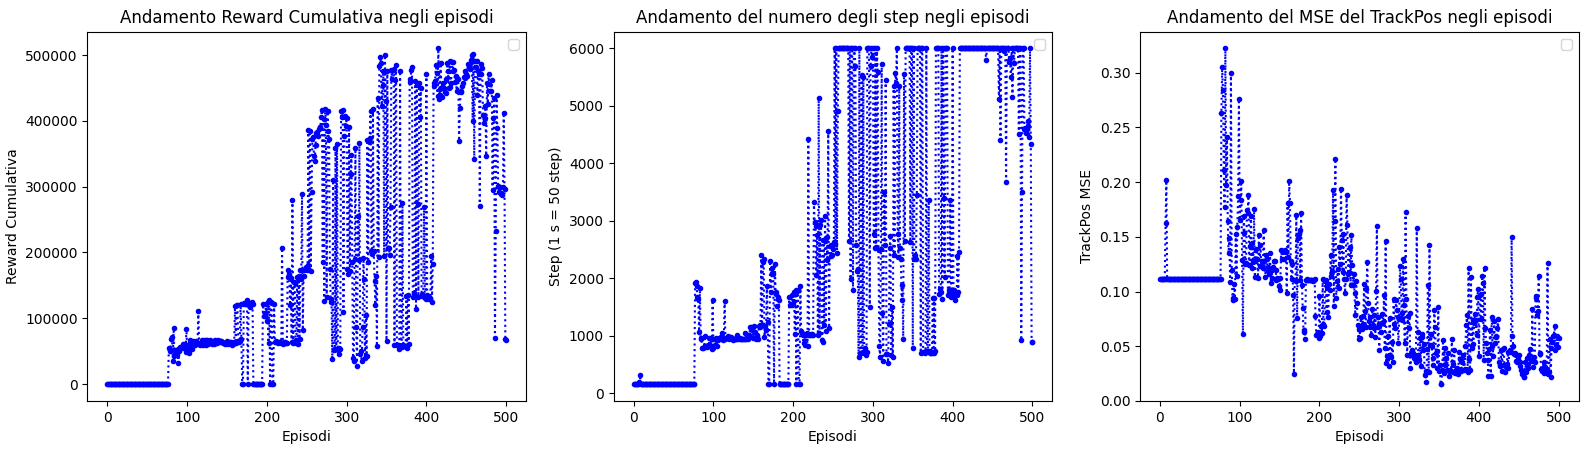
\includegraphics[width = 6in]{Figures/Chapter5/model_1.png}
    \caption{Statistiche del Modello 1}
    \label{fig:model_1}
\end{figure}

\begin{figure}[hb]
    \centering
    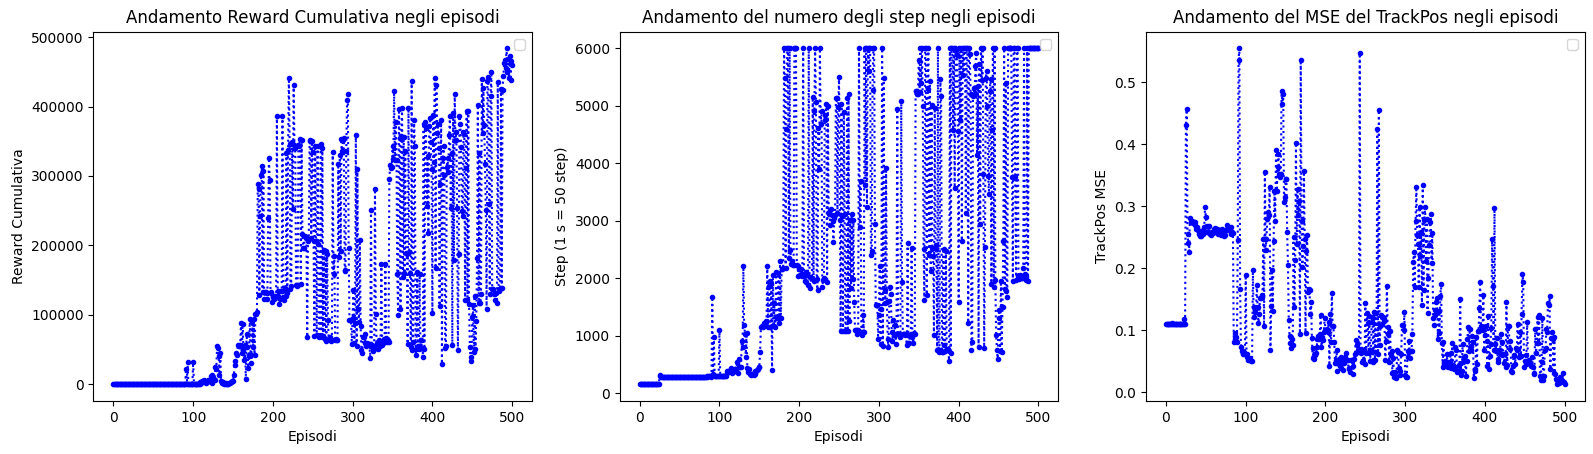
\includegraphics[width = 6in]{Figures/Chapter5/model_2.png}
    \caption{Statistiche del Modello 2}
    \label{fig:model_2}
\end{figure}

\begin{figure}[hb]
    \centering
    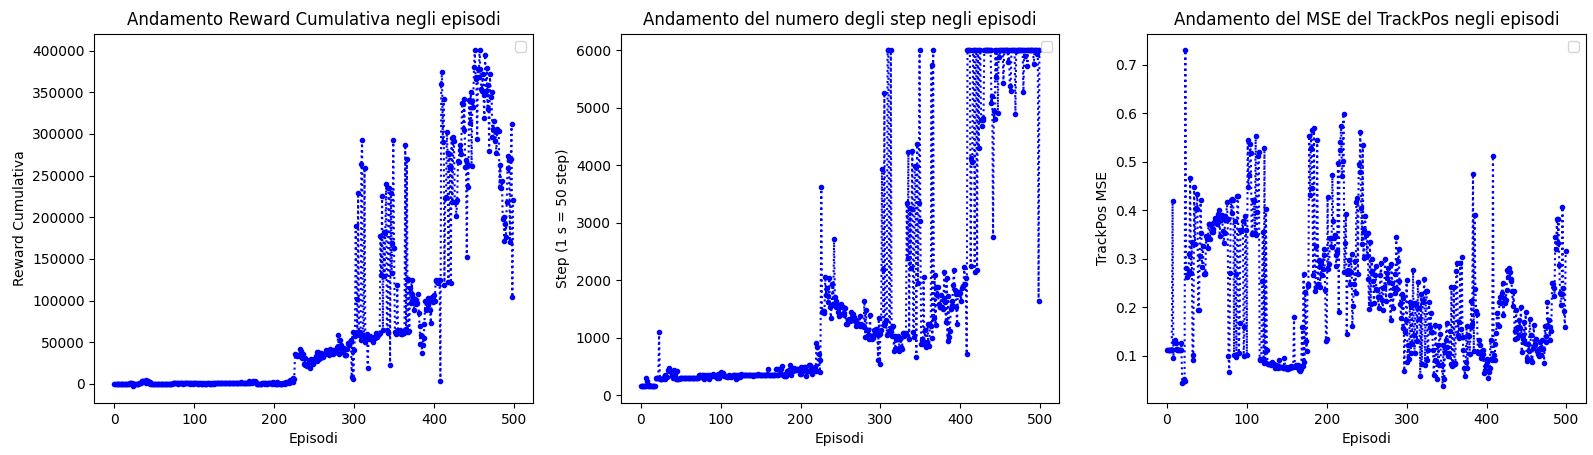
\includegraphics[width = 6in]{Figures/Chapter5/model_3.png}
    \caption{Statistiche del Modello 3}
    \label{fig:model_3}
\end{figure}

\clearpage

\subsection{Test sul tipo di reward function}

Per verificare quale reward function porti risultati migliori, si mettono a paragone i Modelli 1, 4 e 5. Nella fig.\ref{fig:model_4} si mostrano gli andamenti delle metriche del Modello 4, mentre nella fig.\ref{fig:model_5} quelli del Modello 5.

\begin{figure}[hb]
    \centering
    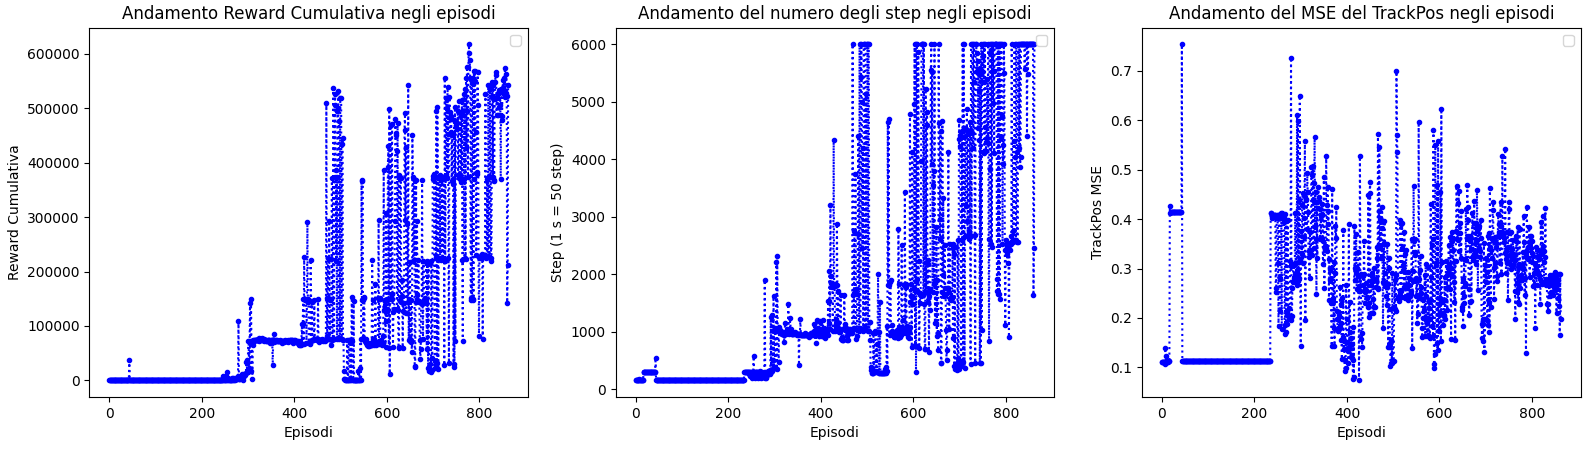
\includegraphics[width = 6in]{Figures/Chapter5/model_4.png}
    \caption{Statistiche del Modello 4}
    \label{fig:model_4}
\end{figure}

\begin{figure}[hb]
    \centering
    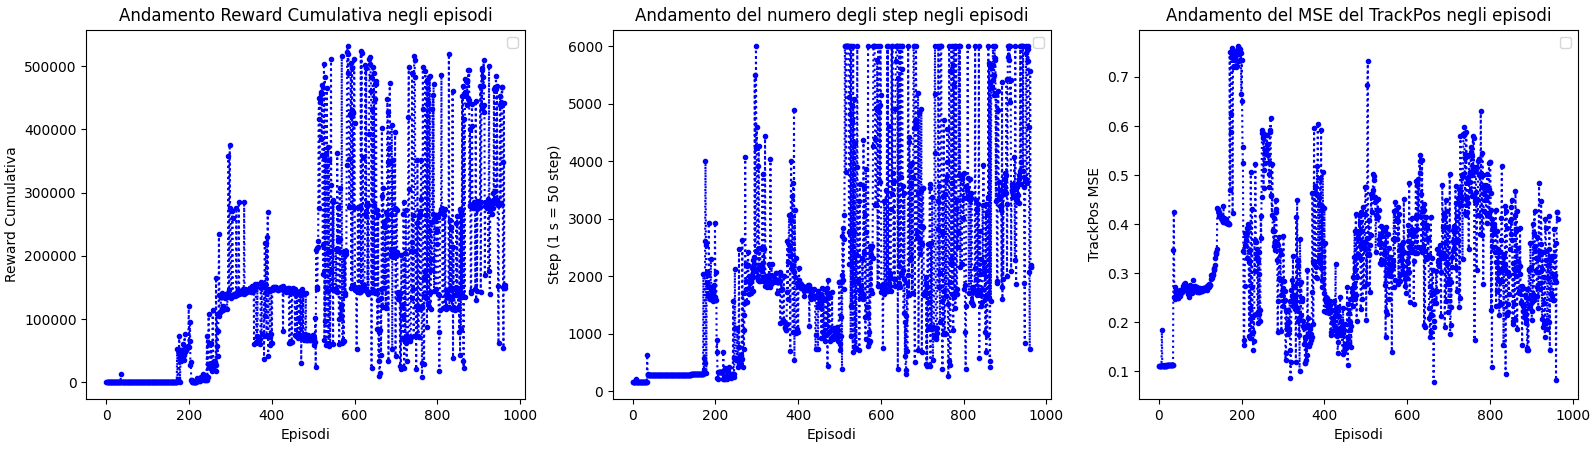
\includegraphics[width = 6in]{Figures/Chapter5/model_5.png}
    \caption{Statistiche del Modello 5}
    \label{fig:model_5}
\end{figure}

Alla fine dei primi 3 passi della valutazione rimangono da confrontare l'episodio 415 del Modello 1, l'episodio 778 del Modello 4 e l'episodio 583 del Modello 5.

\clearpage

Come si nota dalla tab.\ref{tab:models_1-4-5}, i Modelli 4 e 5 hanno una EPISODIC\_REWARD maggiore di quella del Modello 1. Tuttavia si riconosce che il Modello 1 riesce a mantenere un MSE\_TRACKPOS dieci volte più basso rispetto a quello degli altri due modelli.
\newline

Riassumendo, quindi, l'utilizzo di una reward che include il controllo puntuale della trackPos, come quella definita in \ref{rewardfunction}, favorisce l'allenamento di un modello che segue pedissequamente il centro della carreggiata, mentre l'utilizzo di una reward come quelle definite in \ref{rewardfunction_notrackpos} e \ref{rewardfunction_angle} porta all'allenamento di un agente che, seppur mantenendosi sempre entro i limiti della carreggiata, riesce ad elaborare strategie di guida più audaci che portano a ricompense più alte perché è in grado di sfruttatare meglio la conformazione della pista.
\newline

In ultima analisi si osserva che il Modello 5, il quale implementa una reward con controllo sull'angolo del veicolo, ha un MSE\_TRACKPOS maggiore di quello del Modello 4. Questo ci fa concludere che la reward più funzionale alla risoluzione del problema proposto è quella del Modello 4.

\begin{table}[hb]
\centering
\resizebox{\textwidth}{!}{%
\begin{tabular}{|c|c|c|c|c|}
\hline
\multicolumn{1}{|l|}{{\color[HTML]{000000} \textbf{MODEL\_ID}}} &
  {\color[HTML]{000000} \textbf{EPISODIO}} &
  {\color[HTML]{000000} \textbf{EPISODIC\_REWARD}} &
  \multicolumn{1}{l|}{\textbf{MSE\_TRACKPOS}} &
  \multicolumn{1}{l|}{\textbf{N\_STEPS}} \\ \hline
{\color[HTML]{000000} 1} &
  {\color[HTML]{000000} 415} &
  {\color[HTML]{000000} 510353} &
  0,022 &
  6000 \\ \hline
{\color[HTML]{000000} 4} & {\color[HTML]{000000} 778} & {\color[HTML]{000000} 601018} & 0,276 & 6000 \\ \hline
5                        & 583                        & 531486                        & 0,284 & 6000 \\ \hline
\end{tabular}%
}
\caption{Confronto Modelli 1, 4 e 5}
\label{tab:models_1-4-5}
\end{table}

\subsection{Modello finale}

Il Modello 4 e il Modello 5 risultano essere, nel complesso, i due miglior modelli secondo le modalità di confronto definite. Il Modello 4, però, riesce ad ottenere performance molto più alte in termini di EPISODIC\_REWARD, quindi è scelto come modello definitivo nell'episodio 778.
\newline

\clearpage

\section{Risultati numerici}

In questa sezione vengono presentati i risultati numerici ottenuti sul tracciato di validazione dal Modello 4 nell'episodio 778 e confrontati con quelli del Modello 1 nell'episodio 415.
\newline

Nella fig.\ref{fig:model_1-4_reward}, \ref{fig:model_1-4_velocity} e \ref{fig:model_1-4_trackpos} vengono mostrati, rispettivamente, l'andamento della reward, l'andamento della velocità e l'andamento dell'errore quadratico della trackPos dei due modelli nei due rispettivi episodi migliori. Nell'analisi della \ref{fig:model_1-4_trackpos} si tenga presente che il Modello 4 implementa una reward che non impone il mantenimento del centro della carreggiata bensì solo di rimanere all'interno di quest'ultima. Per tale ragione si considera buono ogni risultato minore di 1.

\begin{figure}[hb]
    \centering
    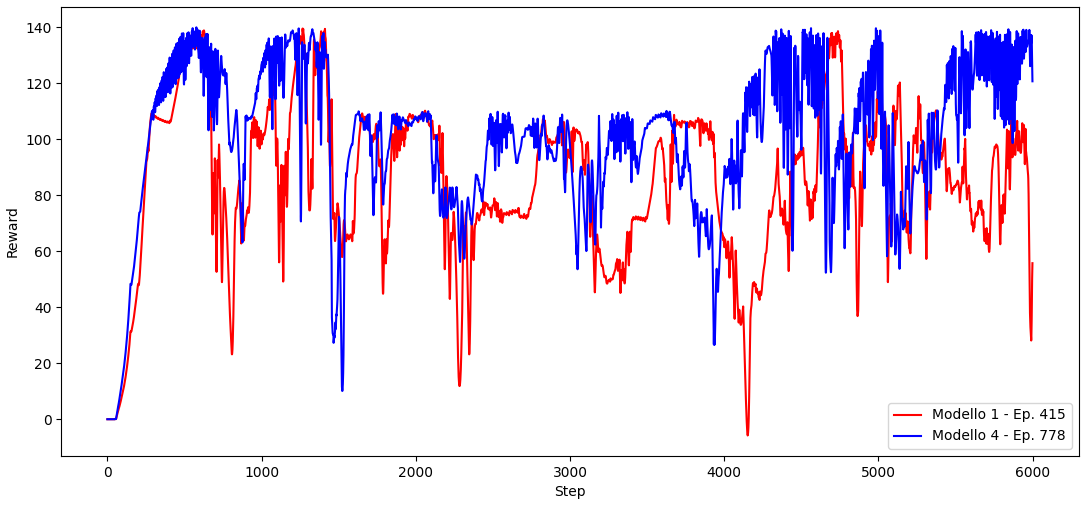
\includegraphics[width = 5.5in]{Figures/Chapter5/model_1-4_reward.png}
    \caption{Reward nell'episodio}
    \label{fig:model_1-4_reward}
\end{figure}

\begin{figure}[hb]
    \centering
    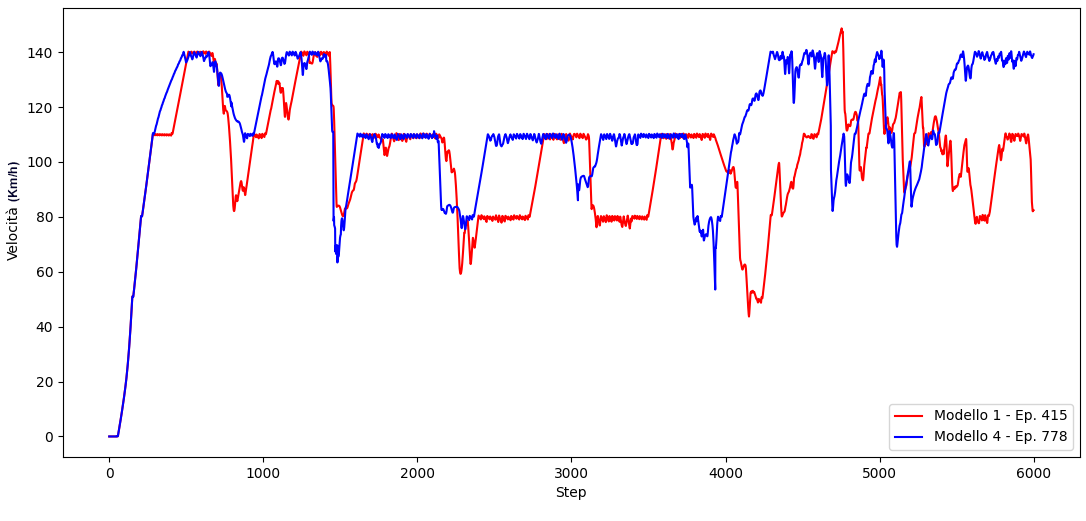
\includegraphics[width = 5.5in]{Figures/Chapter5/model_1-4_velocity.png}
    \caption{Velocità nell'episodio}
    \label{fig:model_1-4_velocity}
\end{figure}

\begin{figure}[hb]
    \centering
    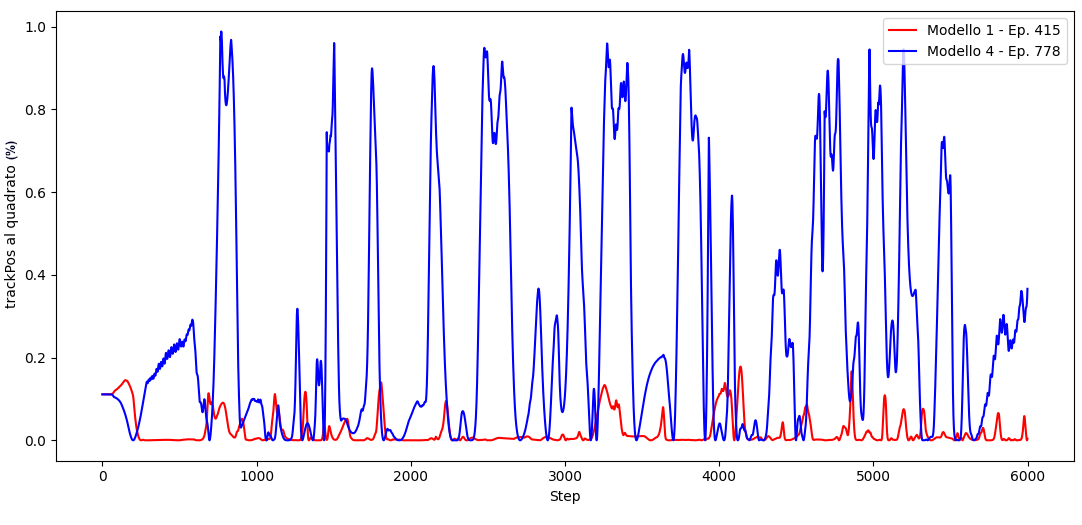
\includegraphics[width = 5.5in]{Figures/Chapter5/model_1-4_trackpos.png}
    \caption{Errore quadratico trackPos nell'episodio}
    \label{fig:model_1-4_trackpos}
\end{figure}
\chapter*{Conclusioni}

In questa tesi ci si è approcciati al problema del lane keeping nell'ambiente di simulazione di guida TORCS utilizzando un approccio di Reinforcement Learning: il DDPG.
\newline

Si è partiti facendo un'introduzione al Reinforcement Learning per poi approdare alle definizioni dei più comuni algoritmi di Deep RL, in cui ricade anche il DDPG. Si è poi presentato nel dettaglio l'ambiente di simulazione TORCS, evidenziandone lati positivi e criticità, le quali hanno avuto bisogno di ulteriori attenzioni sul piano implementativo. Si è spiegata l'importanza del problema del lane keeping nel campo dell'AU e si è utilizzato il DDPG proprio per la creazione di un sistema decisionale end-to-end per la gestione di tale processo nel caso di un veicolo terrestre.
\newline

Infine si sono allenati molteplici modelli e si sono effettuate svariate simulazioni su diverse combinazioni di variazioni parametriche, come il rumore esplorativo e la reward function. Dato che questi test sono stati svolti in un simulatore di gare automobilistiche, ci si è posti il problema di identificare un modello che avesse ottime performance nel mantenimento di carreggiata, senza però mettere in secondo piano la metrica della velocità dell'auto. Per tale ragione il migliore è risultato essere il Modello 4, con reward senza controllo puntuale sulla trackPos e rumore esplorativo Ornstein-Uhlenbeck Mod.
\newline

L'OU si è dimostrato avere performance migliori rispetto alle altre due classi di rumore esplorativo mentre la reward function, caratterizzata dall'avere un maggiore grado di libertà sulla posizione dell'auto in carreggiata, ha permesso di ottenere ottime performance nel caso di applicazione studiato.
\newline

In defintiva il DDPG si è dimostrato essere un validissimo algoritmo per la creazione di un sistema decisionale end-to-end per il lane keeping di un veicolo terrestre.







%%	APPENDIX

%\begin{appendices}

\chapter{Implementazione}

Qui viene fatta una panoramica del codice delle classi e delle procedure essenziali alla realizzazione del progetto.
\newline

Il linguaggio utilizzato è Python 3.7 con il supporto delle librerie \\tensorflow e keras per la creazione e gestione delle reti neurali. Il client utilizzato per l'interazione col server di gioco è SnakeOil\cite{snakeoilWebsite}.

\clearpage

\section{Classe replayBuffer}

\inputminted[
frame=lines,
framesep=2mm,
fontsize=\footnotesize,
linenos
]{python}{Codes/replayBuffer.py}

Questa è la classe che implementa l'experience replay.
\newline

La classe definisce due metodi: uno per salvare una transizione in memoria e un altro per prelevare un batch di transizioni dalla memoria.

\clearpage

\section{Classe Critic}%\label{app:critic}

\inputminted[
frame=lines,
framesep=2mm,
fontsize=\footnotesize,
linenos
]{python}{Codes/critic.py}

La classe Critic racchiude tutti i metodi e le strutture dati per creare, usare e salvare la rete Critic.
\newline

Il cuore della classe è la funzione \textbf{\texttt{create\_critic}}. Essa riceve in ingresso il numero di neuroni del primo e del secondo livello denso nascosto e il learning rate. Nelle \textit{righe 21-23} si crea la parte della rete che prende in input lo stato \textit{s}, mentre nelle \textit{righe 25-26} si osserva la creazione della porzione della rete che lavora con l'azione \textit{a}.
\newline

Nella \textit{riga 28} vengono sommati i risultati intermedi di stato e azione e nella \textit{riga 29-30} si produce il risultato finale: il Q-value.

\clearpage

\section{Classe Actor}%\label{app:actor}

\inputminted[
frame=lines,
framesep=2mm,
fontsize=\footnotesize,
linenos
]{python}{Codes/actor.py}

La classe Actor racchiude tutti i metodi e le strutture dati per creare, usare e salvare la rete Actor.
\newline

La funzione \textbf{\texttt{create\_actor}} crea la rete neurale a partire dalle dimensioni dei due livelli densi nascosti e del learning rate. Si osservi, nelle \textit{righe 26-28} la creazione dei tre neuroni in uscita, fatta ognuna usando una diversa funzione di attivazione contenuta nel file di configurazione del modello.

\clearpage

\section{Classe Rumore}

\subsection{Ornstein-Uhlenbeck modificato}%\label{app:OU}

\inputminted[
frame=lines,
framesep=2mm,
fontsize=\footnotesize,
linenos
]{python}{Codes/ou.py}

\clearpage

Questa classe implementa il primo dei rumori esplorativi utilizzati.
\newline

Questo rumore è una variazione dell'\textit{Ornstein-Uhlenbeck} in quanto, come si vede nella \textit{riga 15}, nel 10\% dei casi viene prodotto un rumore gaussiano con media \textbf{\texttt{MU\textsubscript{2}}} e std \textbf{\texttt{STD\textsubscript{2}}} mentre nel 90\% dei casi viene prodotto un rumore in base al processo stocastico di Ornstein-Uhlenbeck.
\newline

Questo serve a fare in modo che l'agente sia sollecitato con due stimoli molto diversi fra loro in misure diverse. Nove volte su dieci si stimola l'agente ad andare molto veloce attraverso un rumore additivo con media alta sull'accelerazione e nulla sulla frenata e, una volta su dieci, invece, lo si stimola a frenare attraverso un rumore con una media nettamente inferiore sull'accelerazione e alta sulla frenata.
\newline


\clearpage


\subsection{Gaussian Noise}%\label{app:GN}

\inputminted[
frame=lines,
framesep=2mm,
fontsize=\footnotesize,
linenos
]{python}{Codes/gn.py}

Questo rumore è una variazione dell'\textit{$\epsilon$-greedy Gaussian Noise} in quanto, come si vede nella \textit{riga 18}, nel 90\% dei casi viene prodotto un rumore gaussiano con media \textbf{\texttt{MU\textsubscript{1}}} e std \textbf{\texttt{STD\textsubscript{1}}} mentre nel 10\% dei casi uno con media \textbf{\texttt{MU\textsubscript{2}}} e std \textbf{\texttt{STD\textsubscript{2}}}.
\newline

Questo serve a fare in modo che l'agente sia sollecitato con due stimoli molto diversi fra loro in misure diverse. Nove volte su dieci si stimola l'agente ad andare molto veloce attraverso un rumore additivo con media alta sull'accelerazione e nulla sulla frenata e, una volta su dieci, invece, lo si stimola a frenare attraverso un rumore con una media nettamente inferiore sull'accelerazione e alta sulla frenata.
\newline

La probabilità $\epsilon$ viene fatta decadere linearmente in un numero di passi pari a \textbf{\texttt{decay\_time}}.

\clearpage

\subsection{Time Variant Noise}%\label{app:TVNoise}
\inputminted[
frame=lines,
framesep=2mm,
fontsize=\footnotesize,
linenos
]{python}{Codes/tvnoise.py}
\clearpage

Questo classe implementa il TVNoise, un rumore gaussiano con media e std variabile nel tempo.
La classe restituisce un rumore gaussiano con media \textbf{\texttt{MU\textsubscript{1}}} e std \textbf{\texttt{STD\textsubscript{1}}} per i primi \textbf{\texttt{self.time\_step1}} passi.
\newline

Successivamente tende linearmente ad un rumore con distribuzione gaussiana con media \textbf{\texttt{MU\textsubscript{2}}} e std \textbf{\texttt{STD\textsubscript{2}}} in un numero di passi pari a \\\textbf{\texttt{(self.time\_step2 - self.time\_step1)}}.
\newline

Infine, sempre linearmente, tende ad avere media \textbf{\texttt{MU\textsubscript{3}}} e std \textbf{\texttt{STD\textsubscript{3}}} in \textbf{\texttt{(self.time\_step3 - self.time\_step2)}} passi. Nel progetto di tesi questo terzo passaggio viene sfruttato per far decadere a zero linearmente il rumore gaussiano aggiunto.
\newline

Nella fig.\ref{fig:tv_noise_media} viene mostrato un esempio di possibile andamento della media del rumore gaussiano. Lo stesso ragionamento si applica alla std.

\begin{figure}[hb]
    \center
    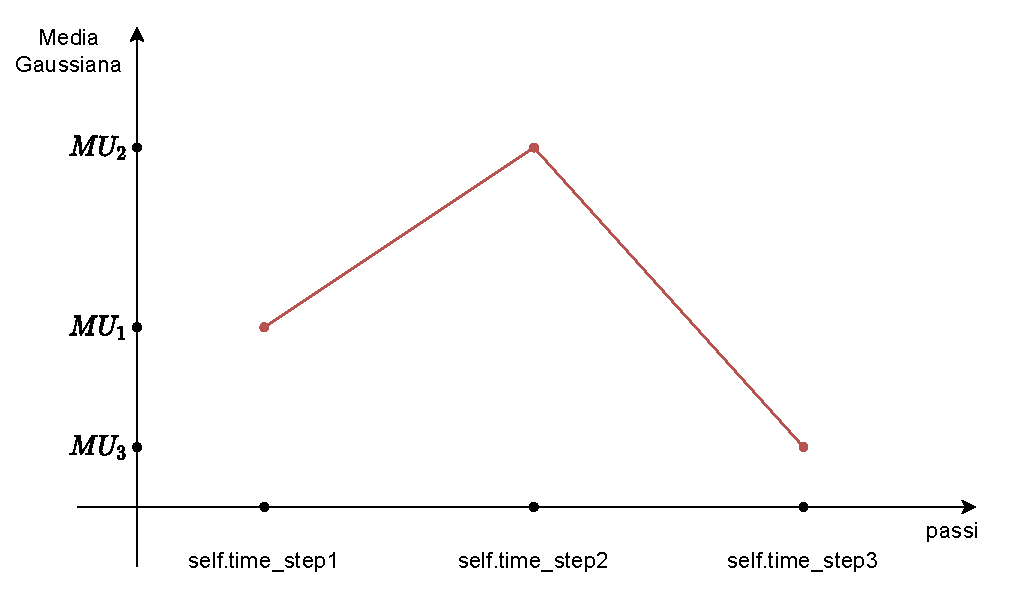
\includegraphics[width = 5in]{Figures/Appendix/tvnoise_media.drawio.pdf}
    \caption{Andamento della media Gaussiana}
    \label{fig:tv_noise_media}
\end{figure}

\clearpage

\section{Funzione train}

\inputminted[
frame=lines,
framesep=2mm,
fontsize=\footnotesize,
linenos
]{python}{Codes/train.py}

\clearpage

La funzione \textbf{\texttt{train}} è il cuore dell'algoritmo di apprendimento. In questa funzione vengono campionate la transizioni dall'experience replay, aggiornati i parametri delle reti Actor e Critic secondo i gradienti e, infine, aggiornate le reti target.
\newline

Nelle \textit{righe 16-28} vengono aggiornati i parametri della rete Critic. In particolare alla \textit{riga 23} viene calcolata la loss di eq.\ref{criticlossddpg} e alle \textit{righe 25-26} ne si calcola il gradiente rispetto ai parametri della rete.
\newline

Nelle \textit{righe 30-39} vengono aggiornati i parametri della rete Actor. Si noti come alla \textit{riga 32} viene invertito il segno ai valori prodotti dal Critic: questo serve poiché l'ottimizzatore utilizzato effettua una discesa del gradiente, quindi invertendo il segno ai valori si effettuerà una salita lungo il gradiente, come imposto dalla eq.\ref{gradactorddpg}. Nella \textit{righe 36-37} viene effettivamente calcolato il gradiente della $Q$ rispetto ai parametri della rete Actor.


\clearpage

\section{Funzione update\_target}

\inputminted[
frame=lines,
framesep=2mm,
fontsize=\footnotesize,
linenos
]{python}{Codes/update_target.py}

La funzione che effettua il soft update delle reti target in ottemperanza alle eq.\ref{ddpgsoftupdate_eq}. Lo \textbf{\texttt{sm\_fact}}, ovvero smooth factor, identifica la $\tau$.

\clearpage

\section{Funzione reward}\label{app:reward}

\subsection{Reward standard}\label{app:reward_standard}

\inputminted[
frame=lines,
framesep=2mm,
fontsize=\footnotesize,
linenos
]{python}{Codes/reward_standard.py}

Codice della reward standard. Restituisce $-200$ se l'agente è fuori carreggiata oppure un numero reale calcolato nella \textit{riga 6}.

\subsection{Reward senza trackPos}\label{app:reward_notrackpos}

\inputminted[
frame=lines,
framesep=2mm,
fontsize=\footnotesize,
linenos
]{python}{Codes/reward_notrackpos.py}

L'unica differenza dalla reward standard è che nella \textit{riga 6} viene rimossa la penalizzazione rispetto alla distanza dal centro della carreggiata. Viene ovviamente mantenuto il controllo di uscita da essa nelle \textit{righe 3-4}.

\subsection{Reward con angle}\label{app:reward_notrackpos_angle}

\inputminted[
frame=lines,
framesep=2mm,
fontsize=\footnotesize,
linenos
]{python}{Codes/reward_notrackpos_angle.py}

Questa reward sostituisce la penalizzazione rispetto alla distanza dal centro della carreggiata con una rispetto all'angolo della vettura rispetto all'asse della carreggiata.

\clearpage


	
\end{appendices}


%%	REFERENCES


\bibliographystyle{plain}
\bibliography{ref}

\end{document}

